% \documentclass[handout]{beamer}
\documentclass{beamer}

%%%%%% Load Packages %%%%%%
\usepackage{xcolor} % font colors
\usepackage{url}
% \usepackage[hidelinks]{hyperref}
\usepackage{minted}
\usepackage{amsmath}
\usepackage{amssymb}
\usepackage{esint} % double surface integrals etc
\usepackage{listings} % like figures but for code
% \usepackage{verbatim}
% \usepackage{fancyvrb}
% \usepackage{enumerate}
\usepackage[shortlabels]{enumitem} % for numbered lists; setlist; shortlabels to define bullet etc.
\usepackage{tikz}
\usepackage{comment} % include block comments
\usepackage{wrapfig} % wrap text around figure 
\usepackage{graphicx}
\usepackage{svg}

%%%%%% Set Theme, Color Scheme %%%%%%
\usetheme{Madrid}

% Change base colour beamer@blendedblue (originally RGB: 0.2,0.2,0.7)
\colorlet{beamer@blendedblue}{green!40!black}

%%%%%% Page Setup %%%%%%
\setbeamersize
{
    text margin left=1cm,
    text margin right=1cm
}

%%%%%% Define Additional Behavior %%%%%%

\AtBeginSection[]
{
  \begin{frame}
    \frametitle{Table of Contents}
    \tableofcontents[currentsection,hideothersubsections]
  \end{frame}
} % displaying table of contents slide with highlight before each section

\setbeamertemplate{caption}[numbered] % number figures in beamer

\definecolor{dgreen}{rgb}{0.,0.6,0.} % define dark green color

\newcommand{\keyw}[1]{\textcolor{dgreen}{\emph{#1}}}
\newcommand{\keytt}[1]{\textcolor{dgreen}{\texttt{#1}}}


% \begingroup\makeatletter\def\@currenvir{verbatim}

\robustify\mintinline % ``helps" with minted???

% \setlist[itemize,1]{label=$\times$}
% \setlist[itemize,2]{label=$\checkmark$}
% \setlist[itemize,3]{label=$\diamond$}
% \setlist[itemize,4]{label=$\bullet$}

%%%%%% Document Title Info %%%%%%

\title{A \LaTeX{} Tutorial}
\author{Lydia England}
% \institute{Overleaf}
\date{2022}

% \usepackage{subfiles}


%%%%%% Document %%%%%%

\begin{document}

\begin{frame}
\titlepage
\end{frame}

\begin{frame}
    \frametitle{Table of Contents}
	\tableofcontents[hideallsubsections]
\end{frame}

%%%%%% Input Files from Elsewhere in the Project %%%%%%
\section{Introduction}
% outline:
%%%%% Pronounciation
%%%%% What is LaTeX?
%%%%% Environment
%%%%% 

% \subsection{What is \LaTeX{}?}
\frame{
\frametitle{Pronunciation Guide}
    \begin{itemize}
        \item[\checkmark] Lah-tek
        \item[\checkmark] Lay-tek
        \item[$\times$] Lay-teks 
    \end{itemize}
}


\begin{frame}[fragile]
\frametitle{Where did \LaTeX{} come from?}
    \textbf{Donald Knuth} designed and wrote TeX in the late 1970s, during revisions of the second volume of his foundational work, \emph{The Art of Computer Programming}; created TeX in response to low-quality typography from publishers. \\ [\baselineskip]
    \emph{TeX} (= Tau Epsilon Chi) is a computer language designed for use in typesetting; in particular, for typesetting math and other technical material. \\[\baselineskip]
    Etymology: \textit{(from Greek ``techne" = art/craft, the stem of `technology') } \\[\baselineskip]
    {\scriptsize\itshape ``Science is knowledge which we understand so well that we can teach it to a computer; and if we don't fully understand something, it is an art to deal with it... In this sense, we should continually be striving to transform every art into a science: in the process, we advance the art." --- Donald Knuth, 1974 Turing Award Lecture}
\end{frame}


\begin{frame}[fragile]
\frametitle{Where did \LaTeX{} come from?}
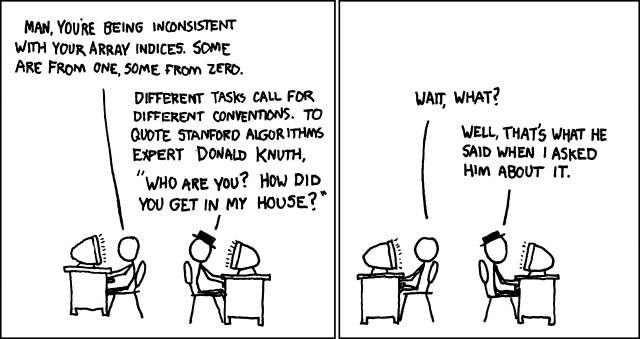
\includegraphics[width=\linewidth]{img/knuth_xkcd.png}
\hspace*{10pt}\hbox{\tiny Alt text: \thinspace{\tiny\itshape His books were kinda intimidating; rappelling down through his skylight seemed like the best option.}} \\
\hspace*{10pt}\hbox{\tiny Image credit:\thinspace{\tiny\itshape \url{https://xkcd.com/163}}} \\
\end{frame}


\frame{
\frametitle{What is \LaTeX{}?}
\LaTeX{} is ... \pause 
\begin{itemize}
    \item A macro package for the TeX programming language \pause
    \item A \textbf{typesetting program} for: \pause
    \begin{itemize}
        \item[$\bullet$] Mathematics \pause
        \item[$\bullet$] Non-Latin scripts (Arabic, Greek, etc.) \pause
    \end{itemize}
    \item Used as a scientific \textbf{document preparation system} for: \pause
    \begin{itemize}
        \item[$\bullet$] STEM Fields (mathematics, physics, computer science, engineering, chemistry, etc.) \pause 
        \item[$\bullet$] non-STEM Fields (economics, linguistics, psychology, philosophy, political science) \pause
    \end{itemize}
\end{itemize}
\begin{exampleblock}{}
    \LaTeX{} lives in between the worlds of \textbf{programming languages} (C, Java, Python, etc.) and \textbf{markup languages} (HTML, XML, etc.). 
\end{exampleblock}
}


\begin{frame}[fragile]
\frametitle{What's special about \LaTeX{}?}
    What separates \LaTeX{} from word processors like Microsoft Word or Google Docs? \pause
    \begin{itemize}
        \item[$\bullet$] \LaTeX{} follows the design principle of separating \emph{content} from \emph{presentation}. \pause
        \item[$\bullet$] The logical \emph{structure} of a document is handled by the author. \pause 
        \item[$\bullet$] Tools like \texttt{chapter, section, table, figure} and more are used to logically structure content without worrying about visual presentation. \pause
        \item[$\bullet$] Manual typesetting is possible, but the majority of adjustments are handled directly by \LaTeX{} itself. \pause
    \end{itemize}
    \vspace{0.1cm}
    \begin{center}
    \Large \LaTeX{} is a \emph{typesetting system}, not a word processor.
    \end{center}
\end{frame}

\begin{frame}[fragile]
\frametitle{Why use \LaTeX{}?}
    With \LaTeX{}, you can... \pause
    \begin{itemize}
        \item[$\bullet$] Create professional looking documents. \pause
        \item[$\bullet$] Create complex documents \emph{fast}. \pause
        \item[$\bullet$] Easily include beautiful mathematical expressions, figures, etc. in a document. \pause
        \item[$\bullet$] Edit images directly at any time. \pause
        \item[$\bullet$] Create dynamic internal references easily. \pause
        \item[$\bullet$] Maintain consistent formatting throughout documents. \pause
        \item[$\bullet$] Focus on content (no more stress about manual formatting!).
    \end{itemize}
\end{frame}

\begin{frame}[fragile]
\frametitle{Why use \LaTeX{}?}
    Learning \LaTeX{} is a little bit like... \\ \pause
    \vspace{0.1cm}
    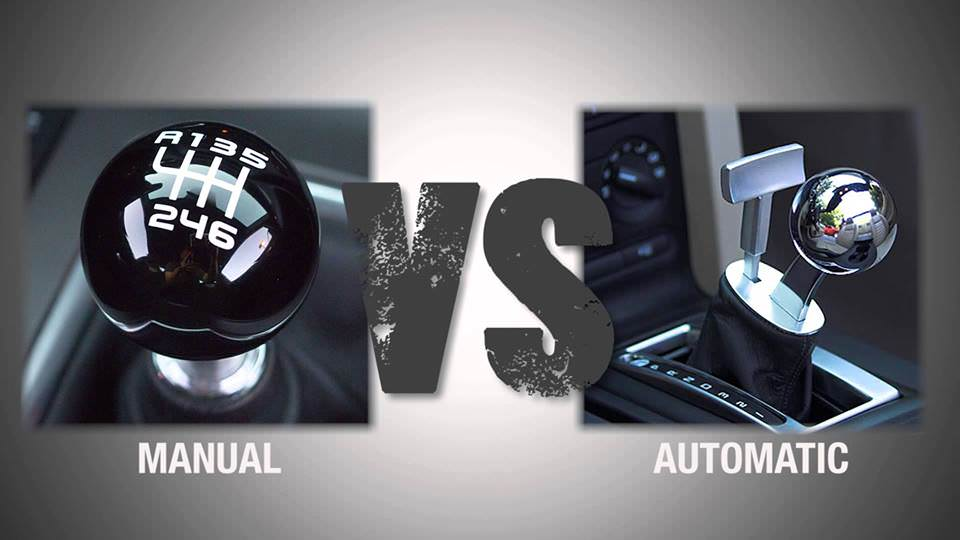
\includegraphics[width=\linewidth]{img/man_auto.jpg}
    \hspace*{15pt}\hbox{\tiny Image credit:\thinspace{\tiny\itshape AIS Insurance Specialists Blog}}
\end{frame}


\begin{frame}[fragile]
\frametitle{Should YOU be using \LaTeX{}?}
    \begin{columns}
    \small
    \column{0.5\linewidth}
        \textbf{You \emph{should} use \LaTeX{} if...} \pause
        \begin{itemize}
            \item[$\bullet$] You work in academia or research. \pause
            \item[$\bullet$] You write documents with lots of equations. \pause
            \item[$\bullet$] You work with long bibliographies. \pause
            \item[$\bullet$] You want to forget about document layout. \pause
            \item[$\bullet$] You want quality {\footnotesize(SVG)} figures. \pause
            \item[$\bullet$] You want forward-compatibility \pause
            \item[$\bullet$] You want your documents to stand out. \pause
        \end{itemize}
    \column{0.5\linewidth}
        \textbf{You should \emph{not} use \LaTeX{} if...} \pause
        \begin{itemize}
            \item[$\bullet$] You don't have time (or the patience) to learn how to use it. \pause
            \item[$\bullet$] You want real-time collaboration with non-\LaTeX{} people. \pause
            \item[$\bullet$] You want to manually control/edit every graphical aspect of a document. \pause
            \item[$\bullet$] You need to exchange working documents with non-\LaTeX{} people. \pause
            \item[$\bullet$] You prefer ``quick and easy." 
        \end{itemize}
    \end{columns}
\end{frame}


\begin{frame}[fragile]
\frametitle{What's \emph{This} Course For?}
    \begin{itemize}[$\bullet$]
        \item Overview of the \LaTeX{} typesetting language.
        \item Demonstrate how to create professional \textit{looking} documents. 
        \item Provide bite-size problems to solve.
    \end{itemize}
\end{frame}




% \subsection{\LaTeX{} Environments}

\begin{frame}
\frametitle{\LaTeX{} Software Packages}
\begin{columns}
\column{0.5\textwidth}
\begin{center}

\includegraphics[width=0.75\textwidth]{img/texlive_logo.png}
{\small \url{https://www.tug.org/texlive/}}

\includegraphics[width=0.5\textwidth]{img/texworks_logo.jpg}
{\small \url{https://tug.org/texworks/}}
\end{center}

\column{0.5\textwidth}
\begin{center}

\includegraphics[width=0.5\textwidth]{img/mactex_logo.png} \\
{\small \url{https://www.tug.org/mactex/}}

\includegraphics[width=0.5\textwidth]{img/texshop_logo.jpg} \\
{\small \url{https://pages.uoregon.edu/koch/texshop/}}
\end{center}
\end{columns}
\end{frame}


\frame{
\frametitle{Cloud-Based \LaTeX{} Editor}
\begin{center}

\includegraphics[width=0.6\linewidth]{img/overleaf_logo.png} \\ 
\url{https://www.overleaf.com} \\
\vspace{1cm}
\begin{exampleblock}{Advantages}
    Many templates, commonly used, collaborative, well-documented and free!
\end{exampleblock}
\end{center}
}


\frame{
\frametitle{Window Layout}
\begin{columns}
\column{0.2\textwidth}
\begin{center}
Files
\end{center}

\column{0.3\textwidth}
\begin{center}
Editor
\end{center}

\column{0.4\textwidth}
\begin{center}
Output Document
\end{center}
\end{columns}

\begin{center}
    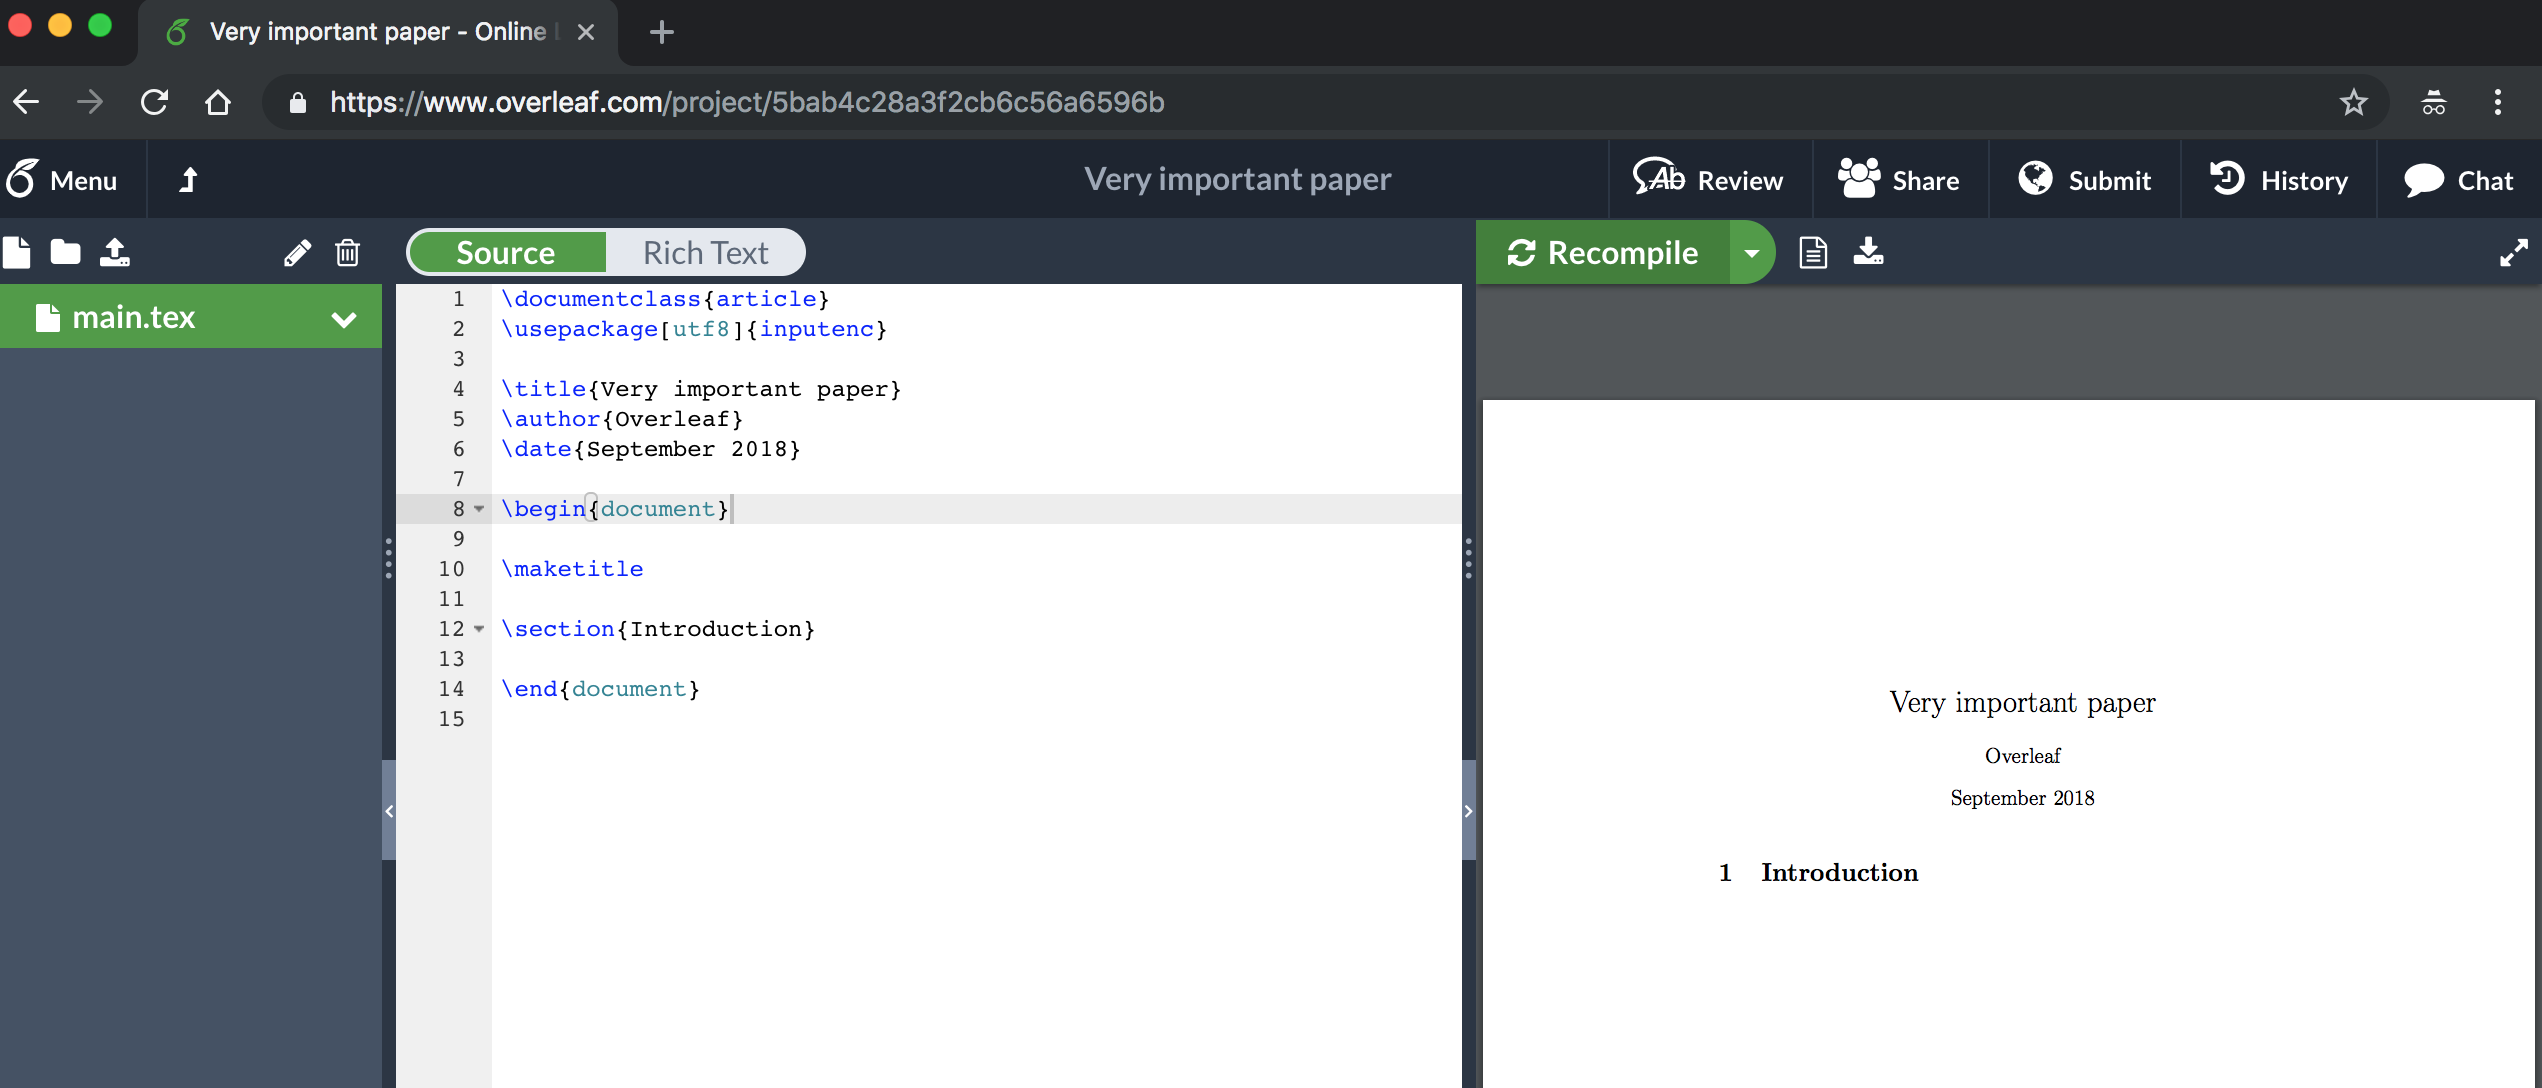
\includegraphics[width=\textwidth]{img/overleaf_windows.png}
\end{center}
}

% {\setbeamercolor{background canvas}{bg=red!15}
% \begin{frame}{This frame is red}
% \end{frame}
% }

% 
% {\setbeamercolor{background canvas}{bg=red!15}
\begin{frame}[fragile]
\frametitle{Exercise: Getting Started \\
{\small Examples and exercises are developed and shown in Overleaf.}} 
\begin{itemize}
    \item[$\bullet$] Open your \LaTeX{} editor of choice.
    \item[$\bullet$] New Project~\rightarrow~Blank Project \rightarrow~\textit{(Title)} 
    \item {\small \textit{This will open a blank project containing the file \texttt{main.tex}.}} 
    \item[$\bullet$] Delete (or comment out) any text and/or commands automatically included in the file.
    \item {\small \textit{We're going to rewrite most of it step-by-step.}} 
\end{itemize}
\begin{alertblock}{}
    \begin{minted}{latex}
    % percentage symbol indicates the start of a  
    % comment.
    % this is a great way to take notes directly 
    % in your document.
    \end{minted}
\end{alertblock}

\end{frame}
% }



\begin{frame}[fragile]
\frametitle{Before we begin:}
\begin{itemize}
    \item[$\bullet$] To comment: \keytt{\% comment text}
    \item Or for longer comments, load \verb|\usepackage{comment}| and use commands \verb|\begin{comment} ... \end{comment}|
    \item[$\bullet$] Compile frequently!
    \item Ctrl + S
    \item Recompile button
    \item For faster compilation, use \textit{Fast (draft) compile mode}.
    \item Recommended to compile from main document.
\end{itemize}
\end{frame}



% {\setbeamercolor{background canvas}{bg=red!15}
\begin{frame}[fragile]
\frametitle{Exercise: Getting Started \\
{\small Examples and exercises are developed and shown in Overleaf.}} 
\begin{itemize}
    \item[$\bullet$] Open your \LaTeX{} editor of choice.
    \item[$\bullet$] New Project~\rightarrow~Blank Project \rightarrow~\textit{(Title)} 
    \item {\small \textit{This will open a blank project containing the file \texttt{main.tex}.}} 
    \item[$\bullet$] Delete (or comment out) any text and/or commands automatically included in the file.
    \item {\small \textit{We're going to rewrite most of it step-by-step.}} 
\end{itemize}
\begin{alertblock}{}
    \begin{minted}{latex}
    % percentage symbol indicates the start of a  
    % comment.
    % this is a great way to take notes directly 
    % in your document.
    \end{minted}
\end{alertblock}

\end{frame}
% }


\section{Document Structure}
% \subsection{Document Components}
\begin{frame}[fragile]
\frametitle{Components of a \LaTeX{} Document}
    \LaTeX{} documents have two primary components: the \keyw{preamble} and the \keyw{body}.\\[\baselineskip] \pause
    In the preamble, the author can set document geometry, load useful packages, define or redefine commands, and more. \\[\baselineskip] \pause
    The actual document content lives in the body of the document. \\[\baselineskip] \pause
    \LaTeX{} file management makes it easy to keep track of document content elements and to reorganize an entire document quickly.
\end{frame}


\begin{frame}[fragile] %{Using \texttt{minted}}
\frametitle{Components of a \LaTeX{} Document: Preamble}
\begin{block}{What is the Preamble?}
    The \emph{preamble} is everything \emph{before} the
    \verb|\begin{document}|
    command. 
    It acts as the document \emph{setup} section.
\end{block} \pause
\begin{block}{Within the Preamble:} 
    \begin{itemize}
        \item[$\bullet$] Define the document \emph{type} \pause
        \item[$\bullet$] Load \textit{packages} \pause
        \item[$\bullet$] Set up document layout, geometry \pause
        \item[$\bullet$] Define title, author, date information \pause
        \item[$\bullet$] Include user-defined macros
    \end{itemize}
\end{block}
\end{frame}


% \begin{frame}[fragile]
% \frametitle{Components of a \LaTeX{} Document: Preamble (Packages)}
    
% \end{frame}


\begin{frame}[fragile]{Using \texttt{minted}}
\frametitle{Preamble Example \#1}
\begin{minted}{latex} 
    \documentclass[12pt, letterpaper]{article}
    \usepackage{geometry}
    \usepackage{amsmath}
    \usepackage[hidelinks]{hyperref}
    \usepackage{tikz}
    \title{My first LaTeX document}
    \author{Jane Doe \thanks{Funded by xxx}}
    \date{August 2022}
    \begin{document}
\end{minted}
\end{frame}

\begin{frame}[fragile]{Using \texttt{minted}}
\frametitle{Preamble Example \#2}
\begin{minted}{latex} 
    \documentclass{beamer}
    \usepackage{url}
    \usepackage{minted}
    \usepackage{listings}
    \usepackage{enumitem}
    \usetheme{Madrid}
    \setbeamersize {
        text margin left=1cm,
        text margin right=1cm }
    \AtBeginSection[] {
      \begin{frame}
        \frametitle{Table of Contents}
        \tableofcontents[currentsection]
      \end{frame} }
    \begin{document}
\end{minted}
\end{frame}

\begin{frame}[fragile]
\frametitle{Components of a \LaTeX{} Document: Body}
\begin{block}{Body}
    The body of a \LaTeX{} document is where all of the text, equations, figures, tables, etc. live.  The body of the document begins with the command \verb|\begin{document}| and ends with the command \verb|\end{document}|.  
\end{block}
\end{frame}



\begin{frame}[fragile]
\frametitle{Components of a \LaTeX{} Document: Multiple Files}
In most \LaTeX{} documents, one has several \keytt{.tex} files --- one for each chapter or section --- joined together into a single output. \pause
\begin{block}{Input other files}
\small
\begin{minted}{latex}
\begin{document}
\input{OtherFile.tex}
\input{AnotherFile.tex}
\end{document}
\end{minted}
\end{block} \pause
\begin{itemize}[$\bullet$]
    \item \LaTeX{} compiles these as if it were one continuous file. \pause
    \item Complex \keytt{Tikz} figures or tables can be written in separate \keytt{.tex} files and loaded at the appropriate places. \pause
    \item Files that are not loaded into \keytt{main}/referenced by other files loaded into \keytt{main} will not be compiled or rendered. \pause
    \item Advantage: Easy to rearrange chapters, sections, etc.
\end{itemize}
\end{frame}

\begin{frame}[fragile]
\frametitle{Components of a \LaTeX{} Document: Summary}
    There are two primary elements of any \LaTeX{} document: the \keyw{preamble}, and the document \keyw{body}. \\[\baselineskip] \pause
    The preamble includes information about the project and its behavior (packages, geometry, user-defined information, commands, aliases, etc.) \\[\baselineskip] \pause
    The body of the document is where everything else (actual output) goes! \\[\baselineskip] \pause
    A \LaTeX{} project can include multiple files; these can be referenced internally and their order can be rearranged.
\end{frame}


% {\setbeamercolor{background canvas}{bg=red!15}
\begin{frame}[fragile]
\frametitle{Exercise: Components \\
{\small Examples and exercises are developed and shown in Overleaf.}} 
\begin{itemize}
    \item[$\bullet$] Open your new project.
    \item[$\bullet$] Enter the following commands into the source code. 
    \item {\small \textit{Feel free to take creative liberties}} 
\end{itemize}
\begin{alertblock}{Build the Preamble}
    \small
    \begin{minted}{latex}
    \documentclass{article}
    \usepackage{geometry}
    \usepackage{amsmath}
    
    \title{Why I Don't Use Microsoft Word}
    \author{Jane Doe}
    \date{November 2022}
    % or: \date{\today}
    \end{minted}
\end{alertblock}

\end{frame}


\begin{frame}[fragile]
\frametitle{Exercise: Components \\
{\small Examples and exercises are developed and shown in Overleaf.}} 
\begin{itemize}
    \item[$\bullet$] Enter the following commands into the source code, following the previous commands. 
    \item {\small \textit{Feel free to take creative liberties}} 
\end{itemize}
\begin{alertblock}{Build the Document Body}
    \small
    \begin{minted}{latex}
    \begin{document}
    
    \maketitle
    
    \section{Introduction}
    In this article, I would like to enumerate for you 
    the ways in which \Latex{} is preferable to ``the 
    word processor who shall not be named."
    
    \end{document}
    \end{minted}
\end{alertblock}

\end{frame}


% }

% \subsection{Basic Structure of a Document}
\begin{frame}[fragile]
\frametitle{Structure: Sections and Chapters}
    \LaTeX{} supports the creation of a dynamic logical document structure and enables customization of sectioning and numbering. \pause
\begin{exampleblock}{}
    \begin{minted}{latex}
    \section{Introduction}
    This is the introduction section. 
    \section{Second Section}
    This is the second section
    \end{minted}
\end{exampleblock} 
\begin{center}
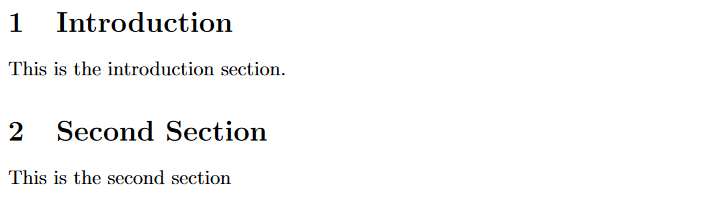
\includegraphics[width=0.8\linewidth]{img/sections_latex.png}
\end{center} \pause
\small For unnumbered sections, add an asterisk; that is, use \verb|\section*{}| instead of \verb|\section{}| and similarly for other sections.
\end{frame}


\begin{frame}[fragile]
\frametitle{Structure: Document Sectioning}
There are up to 7 levels of depth for defining sections depending on the document class. \pause
\begin{exampleblock}{}
    \begin{columns}
        \column{0.1\textwidth}
        -1 \\
        0 \\
        1 \\
        2 \\
        3 \\
        4 \\
        5 \\
        \column{0.7\textwidth}
        \verb|\part{part name}| \\
        \verb|\chapter{chapter name}| \\
        \verb|\section{section name}| \\
        \verb|\subsection{subsection name}| \\
        \verb|\subsubsection{subsubsection name}| \\
        \verb|\paragraph{paragraph name}| \\
        \verb|\subparagraph{subparagraph name}| \\
    \end{columns}
\end{exampleblock} \pause
In most cases, \verb|\section| is the top-level document command. For longer reports or books, \verb|\chapter| or \verb|\part| would be used instead.
\end{frame}


\begin{frame}[fragile]
\frametitle{Structure: The Table of Contents}
The table of contents is easily created with the \keytt{tableofcontents} command. \pause
\begin{exampleblock}{}
    \small
    \begin{minted}{latex}
    \tableofcontents
    \end{minted}
\end{exampleblock} \pause
Sections, subsections, and chapters ARE created in the table of contents; other document levels are NOT. \\[\baselineskip] \pause
Unnumbered sections can be manually added to the table of contents with \verb|\addcontentsline| immediately before the section declaration. \pause
\begin{exampleblock}{}
    \small
    \begin{minted}{latex}
    \addcontentsline{toc}{section}{Unnumbered Section}
    \section*{Unnumbered Section}
    \end{minted}
\end{exampleblock}
\end{frame}


\begin{frame}[fragile]
\frametitle{Structure: The Table of Contents}
The default title for the table of contents is ``Contents," but this is easily changed. \pause
\begin{exampleblock}{}
    \small
    \begin{minted}{latex}
    \renewcommand*\contentsname{Summary}
    \tableofcontents
    \end{minted}
\end{exampleblock} 
\vspace{0.2cm}
This will replace the default name ``Contents" with the new name ``Summary."
\end{frame}


\begin{frame}[fragile]
\frametitle{Structure: Page Numbering}
Page numbers are defined by their \keyw{style} and \keyw{location}. \pause
\begin{itemize}
    \item[$\bullet$] The \keyw{style} is changed with the \verb|\pagenumbering| command. \pause
    \item[$\bullet$] The \keyw{location} and format are changed with the \texttt{fancyhdr} package. \pause
\end{itemize}
\begin{block}{Page Number Styles}
\begin{minted}{latex}
\pagenumbering{⟨style⟩}
\end{minted}
Where \textit{style} is one of the following:
\begin{itemize} \small
    \item \texttt{arabic} (1, 2, 3, ...)
    \item \texttt{alph} (a, b, c, ...)
    \item \texttt{Alph} (A, B, C, ...)
    \item \texttt{roman} (i, ii, iii, ...)
    \item \texttt{Roman} (I, II, III, ...)
\end{itemize}
\end{block}
\end{frame}


\begin{frame}[fragile]
\frametitle{Structure: Page Numbering}
Internally, \LaTeX{} uses a \keyw{counter} to increment and keep track of the current page number. \pause
\begin{block}{Definition: Counter}
    A \emph{counter} is the name of a \LaTeX{} variable used to store an integer number. \LaTeX{} uses counters to internally track numbers of pages, figures, tables, equations, lists, etc. \\
    Internal counters can be manually changed or reset. New counters can be defined by the user.
\end{block} \pause 
The \LaTeX{} page counter variable is called \emph{\keytt{page}}.
\end{frame}


\begin{frame}[fragile]
\frametitle{Structure: Page Numbering}   
\small Counters controlling page numbering can be manually reset with the \keytt{pagenumbering} command at any point in the document. 
\begin{exampleblock}{} 
    \small
    \begin{minted}{latex}
    \pagenumbering{ style }
    \end{minted}
\end{exampleblock} \pause
\small Page number counters can be set to a specific value (\texttt{intval}) with the \keytt{setcounter} command.
\begin{exampleblock}{}
    \small
    \begin{minted}{latex}
    \setcounter{⟨countvar⟩}{⟨intval⟩}
    \end{minted}
\end{exampleblock} \pause
\small To add an amount (\texttt{increment}) to the counter variable (\texttt{countvar}), use the \keytt{addtocounter} command.
\begin{exampleblock}{}
    \small
    \begin{minted}{latex}
    \addtocounter{⟨countvar⟩}{⟨increment⟩}
    \end{minted}
\end{exampleblock} \pause
\small To add 1 to the count variable (\texttt{page}), use the \keytt{stepcounter} command.
\begin{exampleblock}{}
    \small
    \begin{minted}{latex}
    \stepcounter{ countvar }
    \end{minted}
\end{exampleblock} 
\end{frame}


\begin{frame}[fragile]
\frametitle{Structure: Multiple Columns}
\begin{itemize}
    \item[$\bullet$] For simple, two-column documents: pass the parameter \verb|twocolumn| to the initial \verb|documentclass| statement. \pause
    \item[$\bullet$] For more than two columns (or for more flexibility in column layout), use the \verb|multicol| package. \pause
    \item Specify number of columns in the \verb|\begin{multicols}{number of columns}| statement. \pause
    \item Column separation is handled with \verb|\columnsep|. \pause
\end{itemize}
\begin{exampleblock}{}
    \small
    \begin{minted}{latex}
    \usepackage{multicol}
    \setlength{\columnsep}{1cm}
    \end{minted}
\end{exampleblock}
\begin{exampleblock}{}
    \small
    \begin{minted}{latex}
    \begin{multicols}{2}
    Tomorrow, and tomorrow, and tomorrow,
    Creeps in this petty pace from day to day...
    \end{multicols}
    \end{minted}
\end{exampleblock}
\end{frame}


\begin{frame}[fragile]
\frametitle{Structure: Cross-References}
    \begin{wrapfigure}{r}{0.6\textwidth}
       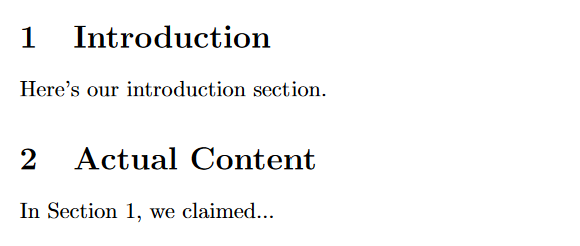
\includegraphics[width=0.58\textwidth]{img/crossrefexample.png}
   \end{wrapfigure}
   \LaTeX{} enables the cross-referencing of numbered items like equations, sections, chapters, figures, and tables internally within a document. \\
   For example, the command \verb|\label{ }| is used to set a label for an item like a section and the command \verb|\ref{ }| is used to reference it by number elsewhere in the document. 
   \small
   \begin{exampleblock}{}
    \begin{minted}{latex}
    \section{Introduction} \label{sec:intro}
    Here's our introduction section. 
    \section{Actual Content} 
    In Section~\ref{sec:intro}, we claimed...
    \end{minted}
   \end{exampleblock}
\end{frame}


% \begin{frame}[fragile]
% \frametitle{Structure: Cross-References}

% \end{frame}


\begin{frame}[fragile]
\frametitle{Structure: Cross-References with Hyperlinks}
To create hyperlinked references, load the \keytt{hyperref} package (optional \keytt{hidelinks} option avoids colored box around hyperlinks):
\begin{exampleblock}{}
\small
\begin{minted}{latex}
\usepackage{hyperref}  
\usepackage[hidelinks]{hyperref}
\end{minted}
\end{exampleblock} \pause
To manually set up link appearance:
\begin{exampleblock}{}
\small
\begin{minted}{latex}
\hypersetup{ ... }     
\end{minted}
\small
\keytt{colorlinks=true} \textit{Links color (default is red)} \\
\keytt{linkcolor=blue} \textit{Internal link color} \\
\keytt{filecolor=magenta} \textit{Local files link color} \\
\keytt{urlcolor=cyan} \textit{Website link color} 
\end{exampleblock} \pause
To keep urls in the same font/style as the rest of the document:
\begin{exampleblock}{}
\small
\begin{minted}{latex}
\urlstyle{same}
\end{minted}
\end{exampleblock}
\end{frame}


\begin{frame}[fragile]
\frametitle{Structure: Hyperlinks}
To link web addresses, use either the \keytt{url} package (displays the url text) or the \keytt{hyperref} package (displays hyperlinked alt text). \pause
\begin{exampleblock}{Example (Hyperlinks and URLs)}
\begin{minted}{latex}
For further reference, see 
\href{https://www.youtube.com/watch?v=dQw4w9WgXcQ}
{A Totally Normal Link} 
or go to the url: 
\url{https://www.youtube.com/watch?v=dQw4w9WgXcQ}
\end{minted}
\end{exampleblock}
\vspace{0.2cm}

\includegraphics[width=\linewidth]{img/hyperlink_ex.png}
\end{frame}



\begin{frame}[fragile]
\frametitle{Structure: More fun structure things!}
\begin{itemize}[$\bullet$]
    \item The \texttt{titlesec} package can be used to customize chapters, sections, subsections etc. \pause
    \item Document class: \texttt{report}. \pause
    \item Document class:  \texttt{book}. \pause
    \item Unbalanced columns. \pause
    \item Floating elements in columns. \pause
    \item Vertical rulers between columns. 
\end{itemize}
\end{frame}


% \begin{frame}[fragile]
% \frametitle{Structures: Summary}

% \end{frame}



% \begin{frame}[fragile]
% \frametitle{Structure: Summary}
    
% \end{frame}


% {\setbeamercolor{background canvas}{bg=red!15}

\begin{frame}[fragile]
\frametitle{Exercise: Structure}
Add the following lines to the preamble of your document. \\
\textit{\small Try to keep the preamble structured logically!}
\begin{alertblock}{Enabling Structure Control from the Preamble}
    \small
    \begin{minted}{latex}
    \usepackage{multicol}
    \usepackage{hyperref}
    % or \usepackage[hidelinks]{hyperref}
    
    \pagenumbering{arabic}
    \setlength{\columnsep}{1cm}

    \renewcommand*\contentsname{Summary}    
    \end{minted}
\end{alertblock}
\end{frame}


\begin{frame}[fragile]
\frametitle{Exercise: Structure} 
\begin{alertblock}{Add Content to Document Body}
    \small
    \begin{minted}{latex}
    \tableofcontents
    
    \section{Introduction} \label{sec:intro}
    In this article, I would like to enumerate for you 
    the ways in which \LaTeX{} is preferable to ``the 
    word processor who shall not be named."

    \subsection{User Interface}
    I haven't decided what to write yet.

    \section{A Brief History}
    In Section~\ref{sec:intro}, I said...
    \end{minted}
\end{alertblock}
\end{frame}


\begin{frame}[fragile]
\frametitle{Challenge: Structure}
\begin{center}
\textbf{Recreate the following document:} \\
\end{center}
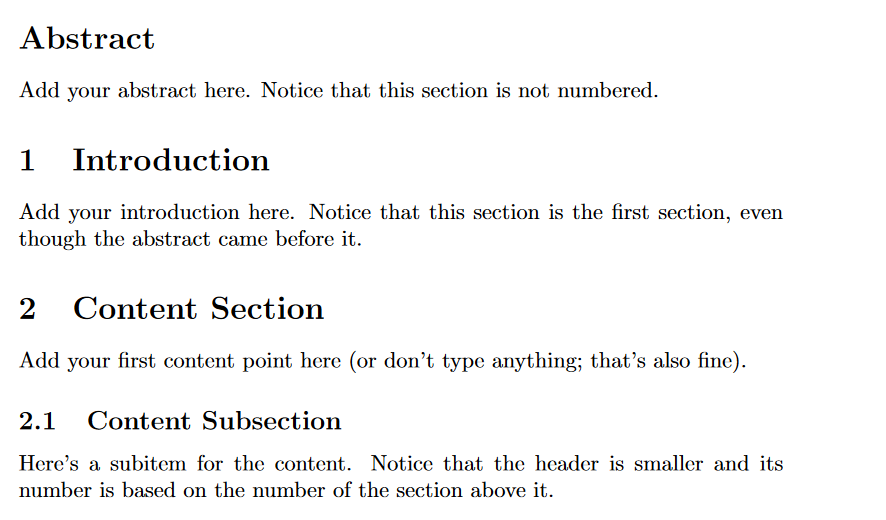
\includegraphics[width=0.9\linewidth]{img/structure_challenge.png}
\end{frame}


\begin{frame}[fragile]
\frametitle{Challenge: Structure}
\begin{alertblock}{Structure Source Code}
\small
\begin{minted}{latex}
\section*{Abstract}
Add your abstract here. 
Notice that this section is not numbered. 
\section{Introduction}
Add your introduction here. 
Notice that this section is the first section, even 
though the abstract came before it.
\section{Content Section}
Add your first content point here 
(or don't type anything; that's also fine).
\subsection{Content Subsection}
Here's a subitem for the content. 
Notice that the header is smaller and its number is 
based on the number of the section above it.
\end{minted}
\end{alertblock}    
\end{frame}


% \begin{frame}[fragile]
% \frametitle{Challenge: Cross-References}
% \begin{center}
%     \textbf{Recreate the following document: }\\
% \end{center}
% \vspace{0.2cm}
% 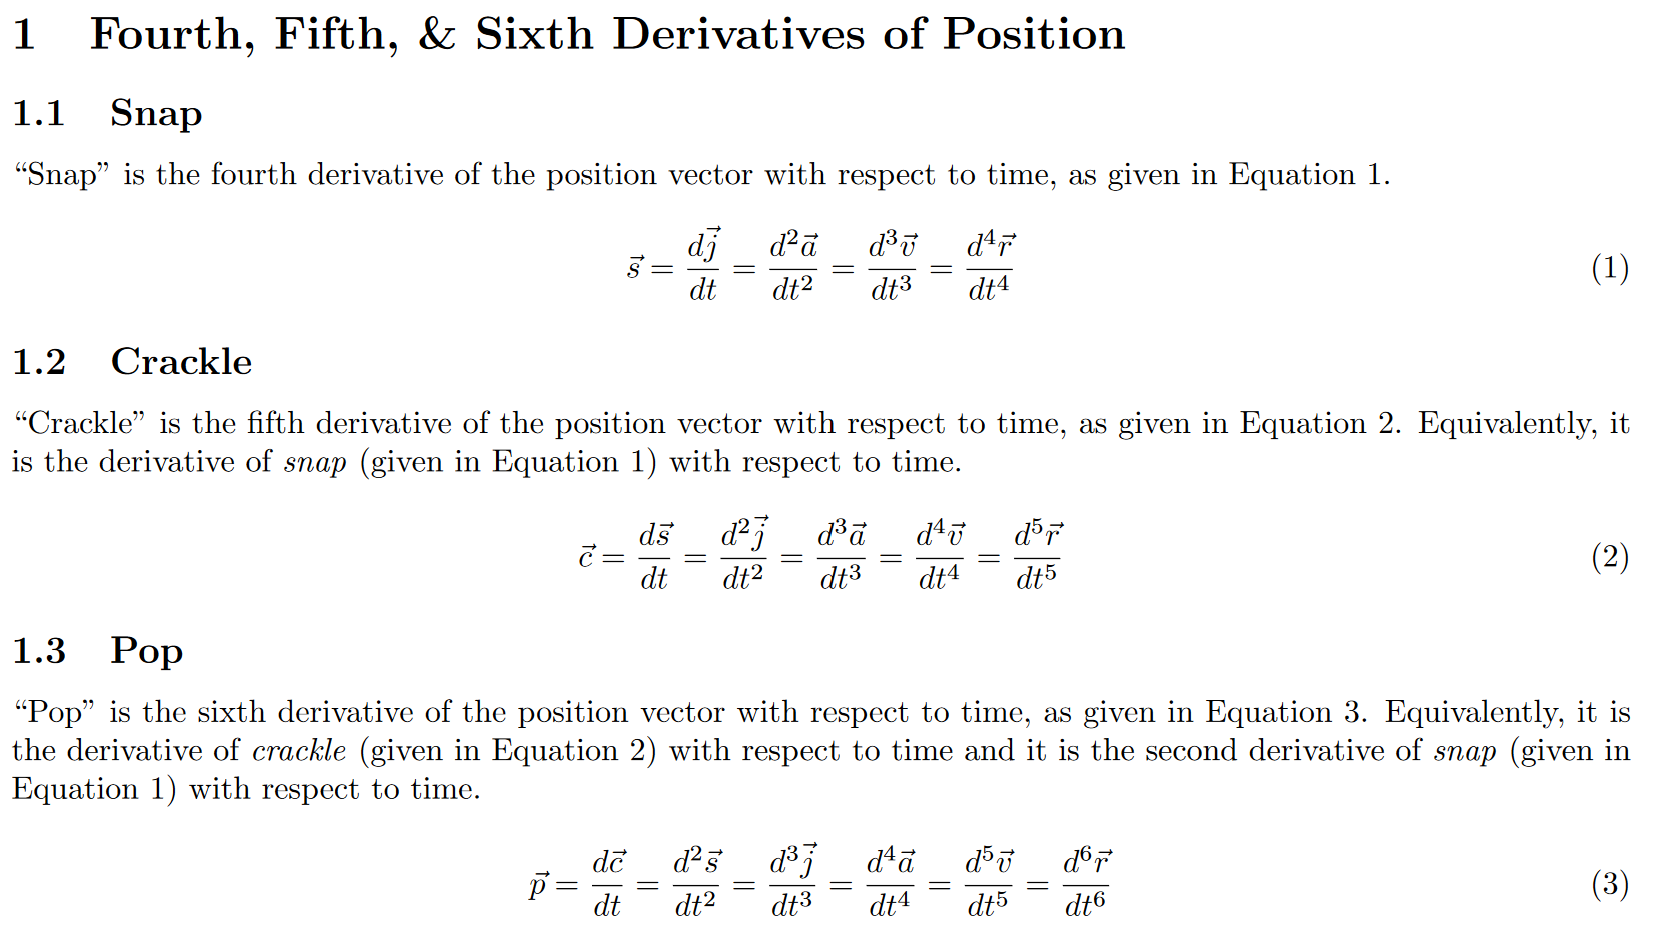
\includegraphics[width=\linewidth]{img/cereal.png}
% \end{frame}


% \begin{frame}[fragile]
% \frametitle{Challenge: Cross-References}
% \begin{alertblock}{Cross-References Source Code (1/3)}
% \small
% \begin{minted}{latex}
% \section{Fourth, Fifth, \& Sixth Derivatives of Position}

% \subsection{Snap} \label{sec:snap}

% ``Snap" is the fourth derivative of the position vector 
% with respect to time, as given in Equation~\ref{eq:snap}.

% \begin{equation} \label{eq:snap}
%     \Vec{s} 
%     = \frac{d\Vec{j}}{dt} = \frac{d^2 \Vec{a}}{dt^2} 
%     = \frac{d^3 \Vec{v}}{dt^3} = \frac{d^4 \Vec{r}}{dt^4}
% \end{equation}
% \end{minted}
% \end{alertblock} 
% \end{frame}




% }


\section{Formatting Basics}
\begin{frame}[fragile]
\frametitle{Lists}
\begin{block}{List Environments in \LaTeX{}}
The \keytt{itemize} environment creates itemized (unordered) lists. \\ \pause
The \keytt{enumerate} environment creates numbered (ordered) lists. \\ \pause
The \keytt{description} environment creates a list of descriptions. \pause
\end{block}
Lists in \LaTeX{} are extremely configurable, enabling a wide variety of list types and structures. \\[\baselineskip] \pause
All lists have the same basic structure:
\begin{exampleblock}{}
\small
\begin{minted}{latex}
\begin{list_type}
   \item {The first item}
   \item The second item 
   \item The third, etc, etc
\end{list_type}
\end{minted}
\end{exampleblock}
\end{frame}


\begin{frame}[fragile]
\frametitle{Lists: Unordered Lists}
\begin{block}{Itemized List}
\begin{minted}{latex}
\begin{itemize}
    \item First unordered list item
    \item Second unordered list item
    \begin{itemize}
        \item Here's an unordered sub-item
    \end{itemize}
\end{itemize}
\end{minted}    
\end{block}
\begin{exampleblock}{}
\begin{itemize}
    \item[$\bullet$] First unordered list item
    \item[$\bullet$] Second unordered list item
    \begin{itemize}
        \item[$-$] Here's an unordered sub-item 
    \end{itemize}
\end{itemize}
\end{exampleblock}
\end{frame}


\begin{frame}[fragile]
\frametitle{Lists: Ordered Lists}
\begin{block}{Enumerated List}
\begin{minted}{latex}
\begin{enumerate}
    \item First ordered list item
    \item Second ordered list item
    \begin{enumerate}
        \item Here's a sub-item
    \end{enumerate}
\end{enumerate}
\end{minted}
\end{block}
\begin{exampleblock}{}
\begin{itemize}
    \item[1.] First ordered list item
    \item[2.] Second ordered list item
    \begin{itemize}
        \item[(a)] Here's a sub-item
    \end{itemize}
\end{itemize}
\end{exampleblock}
\end{frame}


\begin{frame}[fragile]
\frametitle{Lists: Descriptive Lists}
\begin{block}{Descriptive List}
\begin{minted}{latex}
\begin{description}
    \item[Label One] First descriptive list item
    \item[Label Two] Second descriptive list item 
    \begin{description}
        \item[Sub-item Label] Here's a sub-item
    \end{description}
\end{description}
\end{minted}
\end{block}
\begin{exampleblock}{}
\begin{description}
    \item[Label One] First descriptive list item
    \item[Label Two] Second descriptive list item 
    \begin{description}
        \item[Sub-item Label] Here's a sub-item
    \end{description}
\end{description}
\end{exampleblock}
\end{frame}
\subsection{Basic Text Manipulation}
\begin{frame}[fragile]
\frametitle{Basic Text Manipulation with \LaTeX{}}
    \LaTeX{} handles text manipulation and formatting differently than word processors. \\[\baselineskip] \pause
    Instead of editing the output document directly, content is written in plain text and annotated with different commands to indicate styles, sizes, placement, etc. \\[\baselineskip] \pause
    \LaTeX{} takes these commands and compiles the source code into a document. \\[\baselineskip] \pause
    This gives the author significant control over all aspects of the document. \\[\baselineskip]
\end{frame}


\begin{frame}[fragile]
\frametitle{Font Modifiers: Size}
\begin{block}{Optional Arguments in the Preamble}
    \begin{minted}{latex}
    \documentclass[10pt]{article}
    \documentclass[11pt]{article}
    \documentclass[12pt]{article}
    \end{minted}
\end{block} \pause
\begin{block}{Font Modifiers Within Body}
    \begin{columns}
    \column{0.33\textwidth}
    \begin{minted}{latex}
    \tiny
    \scriptsize
    \footnotesize
    \end{minted}
    \column{0.33\textwidth}
    \begin{minted}{latex}
    \normalsize
    \large
    \Large
    \end{minted}
    \column{0.33\textwidth}
    \begin{minted}{latex}
    \LARGE
    \huge
    \HUGE
    \end{minted}
    \end{columns}
\end{block} \pause
Font modifiers act \emph{relative} to the main document font size.
\end{frame}


\begin{frame}[fragile]
\frametitle{Font Modifiers: Size}
Font modifiers can act like a ``switch" to change the font size for all subsequent text within the document, OR font modifiers can act like a ``function" to change the font size for a limited scope. \pause
\begin{block}{Examples}
\footnotesize
\verb|Normal size \LARGE LARGE text| $\to$ Normal size {\Large LARGE text}  \\
\vspace{0.5cm}
\footnotesize
\verb|Normal size {\LARGE LARGE } text| $\to$ Normal size {\Large LARGE} text \\
\vspace{0.5cm}
\end{block} \pause
Other font size packages include: \verb|extsizes|, \verb|anyfontsize|.
\end{frame}


\begin{frame}[fragile]
\frametitle{Font Modifiers: Styles}
\textbf{Bold}, \textit{italic}, and \underline{underline} act on text delimited by \verb|{|, \verb|}|. \pause
\begin{block}{Bold, italic, underline}
    \verb|Normal text| $\to$ Normal text \\ \pause
    \vspace{0.2cm}
    \verb|\textbf{Bold text}| $\to$ \textbf{Bold text} \\ \pause
    \vspace{0.2cm}
    \verb|\textit{Italic text}| $\to$ \textit{Italic text} \\ \pause
    \vspace{0.2cm}
    \verb|\underline{Underlined text}| $\to$ \underline{Underlined text} \\ \pause
\end{block}
These options can be combined. \pause
\begin{block}{Combination Examples}
    \verb|\textbf{textit{Bold italic text}}| $\to$ \textbf{\textit{Bold italic text}} \\
    \vspace{0.2cm}
    \verb|\textbf{textit{\underline{B I U text}}}| $\to$ \textbf{\textit{\underline{B I U text}}} \\
\end{block}
\end{frame}


\begin{frame}[fragile]
\frametitle{Font Modifiers: Styles}
Text emphasis is a content-driven font choice performed by \LaTeX{}. \pause
\begin{block}{Text Emphasis}
    \small
    \verb|Regular \emph{emphasis} text| $\to$ Regular \emph{emphasis} text \\
    \vspace{0.2cm}
    \verb|\textit{Italic \emph{emphasis} text}| $\to$ \textit{Italic} emphasis \textit{text} \\
    \vspace{0.2cm}
    \verb|\emph{Emphatic \emph{emphasis} text}| $\to$ \textit{Emphatic} emphasis \textit{text} \\
    \vspace{0.2cm}
\end{block} \pause
\LaTeX{} chooses the specific emphasis depending on the surrounding text.
\end{frame}


\begin{frame}[fragile]
\frametitle{Font Modifiers: Families}
There are three primary font families available: \textrm{Roman}, \textsf{Sans Serif}, and \texttt{Typewriter}. \pause
\begin{block}{Font Families}
    \verb|\textrm{Default (Roman) Text}| $\to$ \textrm{Default (Roman) Text} \\ \pause
    \vspace{0.2cm}
    \verb|\textsf{Sans Serif Text}| $\to$ \textsf{Sans Serif Text} \\ \pause
    \vspace{0.2cm}
    \verb|\texttt{Typewriter Text}| $\to$ \texttt{Typewriter Text} \\ \pause
    \vspace{0.2cm}
\end{block}
\textrm{Roman} is the default font family. \\ \pause
\texttt{Typewriter text} is a monospaced font used for code snippets (we'll get to those later).
\end{frame}


\begin{frame}[fragile]
\frametitle{Font Modifiers: Colors}
Color manipulation in a \LaTeX{} document uses the \keytt{xcolor} package. There are three additional options which provide more named colors: \pause
\begin{itemize}
    \item \keytt{dvipsnames} loads 68 named colours (CMYK)
    \item \keytt{svgnames} loads 151 named colours (RGB)
    \item \keytt{x11names} loads 317 named colours (RGB) 
\end{itemize} \pause
\begin{exampleblock}{}
\begin{minted}{latex}
\usepackage{xcolor}
\usepackage[dvipsnames]{xcolor}
\usepackage[isvgnames]{xcolor}
\usepackage[x11names]{xcolor}
\end{minted}
\end{exampleblock} \pause
It's also possible to define your own colors! \textit{(But we aren't getting into that right now...)}
\end{frame}


\begin{frame}[fragile]
\frametitle{Font Modifiers: Colors}
The \keytt{dvipsnames} option in the \keytt{xcolor} package provides the the following named colors:\\
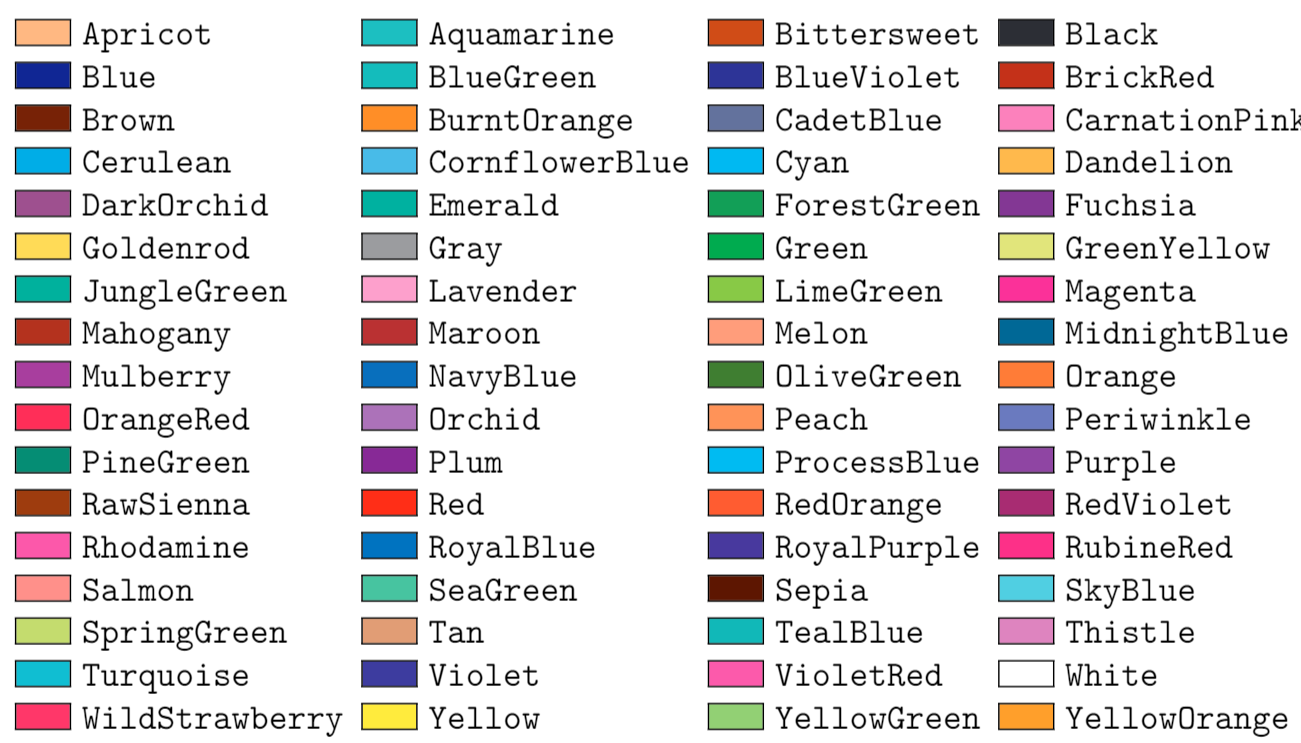
\includegraphics[width=\linewidth]{img/dvipsnamesXcolor.png}
\end{frame}


\begin{frame}[fragile]
\frametitle{Font Modifiers: Colors}
To recolor text, use the \keytt{textcolor} command. 
Its first argument is the desired color; its second is the text to be colored. 
\begin{exampleblock}{}
\begin{minted}{latex}
\textcolor{color}{text}
\end{minted}
\end{exampleblock} \pause
To highlight text in a certain color, use the \keytt{colorbox} command. 
Its first argument is the desired color; its second is the text to be highlighted.
\begin{exampleblock}{}
\begin{minted}{latex}
\colorbox{color}{text}
\end{minted}
\end{exampleblock} \pause
To color an entire page, use the \keytt{pagecolor} command. 
\begin{exampleblock}{}
\begin{minted}{latex}
\pagecolor{color}
\end{minted}
\end{exampleblock}
\end{frame}



\begin{frame}[fragile]
\frametitle{Text Alignment: Justification}
The default justification is \emph{fully justified}. Other justification options include: \pause
\begin{block}{Center Justified Text}
    \begin{minted}{latex}
    \begin{center} ... \end{center}    
    \end{minted}
\end{block} \pause
\begin{block}{Left Justified Text}
    \begin{minted}{latex}
    \begin{flushleft} ... \end{flushleft}    
    \end{minted}
\end{block} \pause
\begin{block}{Right Justified Text}
    \begin{minted}{latex}
    \begin{flushright} ... \end{flushright}    
    \end{minted}
\end{block}
\end{frame}


\begin{frame}[fragile]
\frametitle{Text Alignment: Justification}
\begin{columns} 
    \column{0.5\textwidth}
        {\centering \textbf{Fully Justified Text (Default)}}
            \fbox{\parbox{\textwidth}{\small 
            \vspace{0.35cm}
            Fully justified text is spaced out so that it stretches to fill the entire width of the page. The left and right margins are both perfectly straight.
            \vspace{0.35cm}}} \\ 
    \pause
        \vspace{0.2cm}
        {\centering \textbf{Left Justified Text}}
            \fbox{\parbox{\textwidth}{\small \begin{flushleft} Left justified text is aligned with the left margin. Spacing between words is not stretched; thus, the right margin will have a ragged edge.\end{flushleft}}}
    \pause
    \column{0.5\textwidth}
        {\centering \textbf{Center Justified Text}}
            \fbox{\parbox{\textwidth}{\small \begin{center} Center justified text is aligned down the center of the page. Spacing between words is unstretched; thus, both margins have ragged edges.\end{center}}} \\
    \pause
        \vspace{0.2cm}
        {\centering \textbf{Right Justified Text}}
            \fbox{\parbox{\textwidth}{\small \begin{flushright} Right justified text is aligned with the right margin. Spacing between words is not stretched; thus, the left margin will have a ragged edge.\end{flushright}}}
\end{columns}
\end{frame}


\begin{frame}[fragile]
\frametitle{Text Alignment: Line Breaks}
\begin{block}{Line Breaks}
    \begin{minted}{latex} 
    Here's a line of text. \\
    This is another line of text. \\[\baselineskip]
    ...And another line of text \\[2\baselineskip]
    Here's the last line of text.
    \end{minted}
\end{block}
\vspace{0.4cm}
    \fbox{\parbox{\textwidth}{Here's a line of text. \\
    This is another line of text. \\[\baselineskip]
    ...And another line of text \\[2\baselineskip]
    Here's the last line of text.}}
\end{frame}


\begin{frame}[fragile]
\frametitle{Text Alignment: Indentation}
\LaTeX{} automatically indents new paragraphs. 
\begin{itemize}
    \item[$\bullet$] To skip indentation of a single paragraph: 
    \item \verb|\noindent|
    \item[$\bullet$] To change indentation for the entire document: \verb|\setlength{\parindent}{1cm}|
\end{itemize}
\end{frame}



\begin{frame}[fragile]
\frametitle{Basic Text Manipulation: Summary}
\LaTeX{} allows you to modify... \pause
\begin{itemize}
    \item Text appearance
    \begin{itemize}
        \item Font size (as a ``function" or as a ``switch")
        \item Font style (\textbf{bold}, \textit{italic}, \underline{underline}, \emph{emphasis})
        \item Font family (\textrm{Roman}, \textsf{Sans Serif}, \texttt{Typewriter})
    \end{itemize} \pause
    \item Text alignment
    \begin{itemize}
        \item Justification (left, right, center, fully justified)
        \item Line breaks (single or multiple lines)
        \item Indentation \small (\verb|\noindent| or \verb|\setlength{\parindent}{...}|
    \end{itemize} \pause
\end{itemize}
... and more!
\end{frame}


% {\setbeamercolor{background canvas}{bg=red!15}

\begin{frame}[fragile]
\frametitle{Challenge: Font Styles}
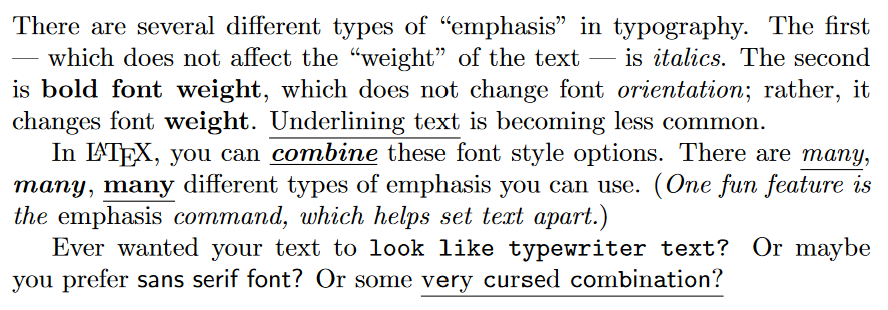
\includegraphics[width=\linewidth]{img/FontEmphs.png}
\end{frame}


\begin{frame}[fragile]
\frametitle{Challenge: Font Styles}
\begin{alertblock}{Font Styles: Source Code (1/3)}
\small
\begin{minted}{latex}
There are several different types of ``emphasis" in 
typography.
The first --- which does not affect the ``weight" of the
text --- is \textit{italics}.
The second is \textbf{bold font weight}, which does not 
change font \textit{orientation}; rather, it changes font
\textbf{weight}.
\underline{Underlining text} is becoming less common.
\end{minted} 
\end{alertblock}
\end{frame}


\begin{frame}[fragile]
\frametitle{Challenge: Font Styles}
\begin{alertblock}{Font Styles: Source Code (2/3)}
\small
\begin{minted}{latex}
In \LaTeX{}, you can \textit{\textbf{\underline{combine}}}
these font style options. 
There are \textit{\underline{many}}, 
\textbf{\textit{many}}, \textbf{\underline{many}} 
different types of emphasis you can use. 
(\textit{One fun feature is the \emph{emphasis} command, 
which helps set text apart.})
\end{minted} 
\end{alertblock}
\end{frame}


\begin{frame}[fragile]
\frametitle{Challenge: Font Styles}
\begin{alertblock}{Font Styles: Source Code (3/3)}
\small
\begin{minted}{latex}
Ever wanted your text to \texttt{look like typewriter 
text?} Or maybe you prefer \textsf{sans serif font?} Or
some \underline{\textrm{v}\texttt{e}\textsf{r}\textrm{y} 
\texttt{c}\textsf{u}\textrm{r}\texttt{s}\textsf{e}
\textrm{d} \texttt{c}\textsf{o}\textrm{m}\texttt{b}
\textsf{i}\textrm{n}\texttt{a}\textsf{t}\textrm{i}
\texttt{o}\textsf{n}\textrm{?}}
\end{minted}
\end{alertblock}
\end{frame}


\begin{frame}[fragile]
\frametitle{Exercise: Font Colors}
Add the following line to the preamble of your document. \\
\textit{\small Try to keep the preamble structured logically!}
\begin{alertblock}{}
\small
\begin{minted}{latex}
\usepackage{xcolor}   
\end{minted}
\end{alertblock}
\end{frame}


\begin{frame}[fragile]
\frametitle{Challenge: Font Colors}
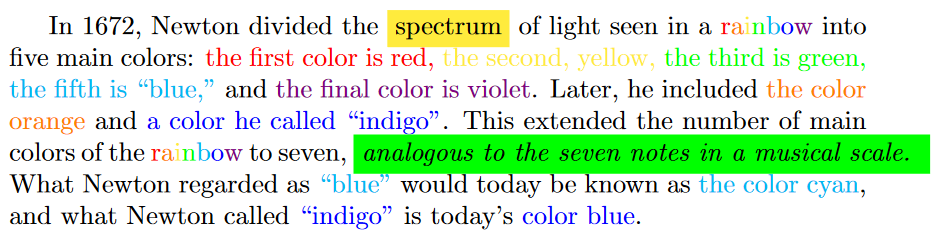
\includegraphics[width=\linewidth]{img/colorsChallenge.png}
\end{frame}


\begin{frame}[fragile]
\frametitle{Challenge: Font Colors}
\begin{alertblock}{Font Colors: Source Code (1/2)}
\small
\begin{minted}{latex}
In 1672, Newton divided the \colorbox{yellow}{spectrum} of 
light seen in a \textcolor{red}{r}\textcolor{orange}
{a}\textcolor{yellow}{i}\textcolor{green}
{n}\textcolor{cyan}{b}\textcolor{blue}
{o}\textcolor{violet}{w} into five main colors: 
\textcolor{red}{the first color is red,} 
\textcolor{yellow}{the second, yellow,} 
\textcolor{green}{the third is green,} 
\textcolor{cyan}{the fifth is ``blue,"} and 
\textcolor{violet}{the final color is violet}.
Later, he included \textcolor{orange}{the color orange} 
and \textcolor{blue}{a color he called ``indigo"}. 
\end{minted} 
\end{alertblock}
\end{frame}

\begin{frame}[fragile]
\frametitle{Challenge: Font Colors}
\begin{alertblock}{Font Colors: Source Code (2/2)}
\small
\begin{minted}{latex}
This extended the number of main colors of the 
\textcolor{red}{r}\textcolor{orange}{a} 
\textcolor{yellow}{i}\textcolor{green}{n} 
\textcolor{cyan}{b}\textcolor{blue}{o} 
\textcolor{violet}{w} to seven, \colorbox{green}
{\textit{analogous to the seven notes in a musical scale.}}
What Newton regarded as \textcolor{cyan}{``blue"} would 
today be known as \textcolor{cyan}{the color cyan}, and 
what Newton called \textcolor{blue}{``indigo"} is today's  
\textcolor{blue}{color blue}.
\end{minted} 
\end{alertblock}
\end{frame}



% }

\subsection{Basic Math Notation}
\begin{frame}[fragile]
\frametitle{Basic Math Notation with \LaTeX{}}
Typesetting mathematical expressions is one of \LaTeX{}'s greatest strengths --- and one of the primary motivations which drove Donald Knuth to develop the original TeX system. \\[\baselineskip]
\LaTeX{} provides thousands of different mathematical symbols and supports multiple different math environments. \\[\baselineskip]
\LaTeX{} is the mathematical typesetting standard in all technical disciplines and in many related fields.
\end{frame}

\begin{frame}[fragile]
\frametitle{Math Modes}
\begin{columns}
\column{0.5\textwidth}
\begin{center}
    \textbf{Display Style Math Mode} \\
    \textit{Puts math on display} \\
    \vspace{0.4cm}
    \fbox{\parbox{\textwidth}{\small It follows that
    \begin{align}
        T(\Vec{u}) & = \sum^n_{j=1} \sum^m_{k=1} M_{jk} x_k \Vec{w}_j 
    \end{align}
    Examination of this formula shows that
    \[y_j = \sum^m_{k=1} M_{jk} x_k\]
    }}
\end{center}

\column{0.5\textwidth}
\begin{center}
    \textbf{Inline (text) Style Math Mode} \\
    \textit{Math stays in the line} \\
    \vspace{0.4cm}
     \fbox{\parbox{\textwidth}{\small But if $T: V \to W$ is a linear transformation then $T(\vec{u}) = T(x_1 \Vec{v}_1 + x_2 \Vec{v_2} + ... + x_m \Vec{m})$. 
     Moreover, because we know that \(T(\Vec{v}_1), T(\Vec{v}_2),...,T(\Vec{v}_m)\) are the elements of the vector space \(W\), we can therefore write 
        \(T(\Vec{v}_k) = \sum^n_{j=1} M_{jk} \Vec{w}_j \) where the quantities \(M_{jk}\) are scalars. \\[\baselineskip]
    }}
\end{center}
\end{columns}
\end{frame}



\begin{frame}[fragile]
\frametitle{Math Modes: Display} 
% \textbf{Display Style Math Mode} \\
\begin{block}{Delimiters for Display Math Mode}
\small
Primary delimiters: \verb|\begin{displaymath} ... \end{displaymath}| \\
Short form \LaTeX{} delimiters: \verb|\[ ... \]| \\
Short form TeX delimiters: \verb|$$ ... $$| \\
\end{block}
\begin{exampleblock}{}
\small
\begin{minted}{latex}
    \[ \iiint\limits_S dV 
        =   \int^{2\pi}_{\phi=0}
            \int^{\pi}_{\theta=0}  
            \int^{r}_{\rho=0} 
            \rho^2 d\cos{\theta} d\phi \]
\end{minted}
    \[ \iiint\limits_S dV = \int^{2\pi}_{\phi=0} \int^{\pi}_{\theta=0} \int^{r}_{\rho=0} \rho^2 d\cos{\theta} d\phi \]
\end{exampleblock}
\end{frame}


\begin{frame}[fragile]
\frametitle{Math Modes: Inline} 
% \textbf{Display Style Math Mode} \\
\begin{block}{Delimiters for Inline Math Mode}
\small
Primary delimiters: \verb|\begin{math} ... \end{math}| \\
Short form \LaTeX{} delimiters: \verb|\( ... \)| \\
Short form TeX delimiters: \verb|$ ... $| \\
\end{block}
% \textbf{Example:} 
\vspace{0.3cm}
\small
\begin{minted}{latex}
\( p(x) = a_n x^n + a_{n-1} x^{n-1} + a_{n-2} x^{n-2} 
        + ... + a_2 x^2 + a_1 x + a_0 \)

$c^2 = a^2 + b^2 - 2ab\cos{\theta}$
\end{minted}
\vspace{0.3cm}
\( p(x) = a_n x^n + a_{n-1} x^{n-1} + a_{n-2} x^{n-2} 
        + ... + a_2 x^2 + a_1 x + a_0 \) \\[\baselineskip]
\vspace{0.3cm}
$c^2 = a^2 + b^2 - 2ab\cos{\theta}$
\end{frame}


\begin{frame}[fragile]
\frametitle{Math Modes: Which one should you use?}
\begin{columns}
    \column{0.5\linewidth}
    \textbf{Use display style math when...}
    \begin{itemize}
        \item[$\bullet$] The mathematical expression is set apart from the main text
        \item[$\bullet$] You want to number an equation (and possibly label and reference it later in the document)
    \end{itemize}
    \column{0.5\linewidth}
    \textbf{Use inline style math when...}
    \begin{itemize}
        \item[$\bullet$] The mathematical expression is included within a line or paragraph of text
        \item[$\bullet$] You are referencing a variable in a line of text (i.e., ``We have the variables $x$, $y$, and $z$)
    \end{itemize}
\end{columns}
\begin{block}{Change style within mode}
Force display math in inline mode: \verb|\( \displaymath ... \)| \\
Force inline style math in display mode: \verb|\[ \textstyle ... \]| \\
\end{block}
\end{frame}


\begin{frame}[fragile]
\frametitle{Math Modes: Examples}
\begin{exampleblock}{Display Style / Inline Mode}
    \small The Basel problem is the problem of computing the sum of the squares of the reciprocals of natural numbers. It turns out that \( \displaystyle \sum^\infty_{n=1} \frac{1}{n^2} = \frac{\pi^2}{6}\). In 1735, Euler proved this result.
\end{exampleblock}
\begin{exampleblock}{Inline Style / Inline Mode}
    \small The Basel problem is the problem of computing the sum of the squares of the reciprocals of natural numbers. It turns out that \( \sum^\infty_{n=1} \frac{1}{n^2} = \frac{\pi^2}{6}\). In 1735, Euler proved this result.
\end{exampleblock}
\end{frame}

\begin{frame}[fragile]
\frametitle{Math Modes: Examples}
\begin{exampleblock}{Inline Style / Display Mode}
    \small The Basel problem is the problem of computing the sum of the squares of the reciprocals of natural numbers. It turns out that \[ \textstyle \sum^\infty_{n=1} \frac{1}{n^2} = \frac{\pi^2}{6}\] In 1735, Euler proved this result.
\end{exampleblock}
\begin{exampleblock}{Display Style / Display Mode}
    \small The Basel problem is the problem of computing the sum of the squares of the reciprocals of natural numbers. It turns out that \[ \sum^\infty_{n=1} \frac{1}{n^2} = \frac{\pi^2}{6}\] In 1735, Euler proved this result.
\end{exampleblock}
\end{frame}


\begin{frame}[fragile]
\frametitle{Math Modes: \texttt{amsmath} Package}
\begin{itemize}
    \item[$\bullet$] Developed for the American Mathematical Society (AMS)
    \item[$\bullet$] Principle package of the AMS-\LaTeX{} distribution
    \item[$\bullet$] Provides additional features to facilitate mathematical typesetting
    \item[$\bullet$] \textit{You should be using this package in any document with mathematical notation} 
    \item[$\bullet$] \verb|\usepackage{amsmath}|
\end{itemize}
% \begin{centering}
% 
\includegraphics[width=0.5\linewidth]{img/ams_logo.png}
% \end{centering}
\tikz[remember picture, overlay] {\node[anchor=south east, outer sep=15pt] at (current page.south east) {
\includegraphics[width=5cm]{img/ams_logo.png}};}
\end{frame}



\begin{frame}[fragile]
\frametitle{Math Modes: \texttt{amsmath} Package} 
\begin{block}{Writing a Single Equation}
    \verb|\begin{equation} ... \end{equation}| \\
\end{block}
To write an equation, use the \verb|\equation| or \verb|\*equation| environment depending on if you want your equation numbered. % Additionally, labels can be added with \verb|\label{}| to reference the equation later within the document.
\begin{exampleblock}{Example}
\small
\begin{minted}{latex}
\begin{equation} \label{eu_eqn}
e^{\pi i} + 1 = 0
\end{equation}

The beautiful equation \ref{eu_eqn} is known as the Euler
equation.
\end{minted}
\begin{equation} \label{eu_eqn}
e^{\pi i} + 1 = 0
\end{equation}

The beautiful equation~\ref{eu_eqn} is known as the Euler
equation.
\end{exampleblock}
\end{frame}



\begin{frame}[fragile]
\frametitle{Math Modes: \texttt{amsmath} Package} 
\begin{block}{Displaying Long Equations}
    \verb|\begin{multline} ... \end{multline}| \\
\end{block}
For equations longer than a line, use the \verb|multline| or \verb|multline*| environment. Use a double backslash to indicate where the equation should be broken.
\begin{exampleblock}{Example}
\small
\begin{minted}{latex}
\begin{multline*}
p(x) = 3x^6 + 14x^5y + 590x^4y^2 + 19x^3y^3\\ 
- 12x^2y^4 - 12xy^5 + 2y^6 - a^3b^3
\end{multline*}
\end{minted}
\begin{multline*}
p(x) = 3x^6 + 14x^5y + 590x^4y^2 + 19x^3y^3\\ 
- 12x^2y^4 - 12xy^5 + 2y^6 - a^3b^3
\end{multline*}
\end{exampleblock}
\end{frame}


\begin{frame}[fragile]
\frametitle{Math Modes: \texttt{amsmath} Package} 
\begin{block}{Splitting and Aligning an Equation }
\small
\verb|\begin{equation}\begin{split} ... \end{split}\end{equation}| \\
\end{block}
\verb|Split| is similar to \verb|multline|. It is used to break an equation and align it in columns. It is used within an \verb|equation| environment. 
\begin{exampleblock}{Example}
\small
\begin{minted}{latex}
\begin{equation} \begin{split}
A & = \frac{\pi r^2}{2} \\
 & = \frac{1}{2} \pi r^2
\end{split} \end{equation}
\end{minted}
\begin{equation} \begin{split}
A & = \frac{\pi r^2}{2} \\
 & = \frac{1}{2} \pi r^2
\end{split} \end{equation}
\end{exampleblock}
\end{frame}


\begin{frame}[fragile]
\frametitle{Math Modes: \texttt{amsmath} Package} 
\begin{block}{Aligning Several Equations}
\small
\verb|\begin{align} ... \end{align}| \\
\end{block}
To align several equations vertically, use the \verb|align| environment. The ampersand character \& determines where equations align.
\begin{exampleblock}{Example}
\small
\begin{minted}{latex}
\begin{align*}
x&=y           &  w &=z              &  a&=b+c\\
-4 + 5x&=2+y   &  w+2&=-1+w          &  ab&=cb
\end{align*}
\end{minted}
\begin{align*}
x&=y           &  w &=z              &  a&=b+c\\
-4 + 5x&=2+y   &  w+2&=-1+w          &  ab&=cb
\end{align*}
\end{exampleblock}
\end{frame}


\begin{frame}[fragile]
\frametitle{Math Modes: \texttt{amsmath} Package} 
\begin{block}{Grouping and Centering Equations}
\small
\verb|\begin{align} ... \end{align}| \\
\end{block}
To display a set of consecutive equations, centered, with no alignment, use the \verb|gather| environment.
\begin{exampleblock}{Example}
\small
\begin{minted}{latex}
\begin{gather*} 
2x - 5y =  8 \\ 
3x^2 + 9y =  3a + c
\end{gather*}
\end{minted}
\begin{gather*} 
2x - 5y =  8 \\ 
3x^2 + 9y =  3a + c
\end{gather*}
\end{exampleblock}
\end{frame}


\begin{frame}[fragile]
\frametitle{Math Modes: \texttt{amsmath} Package} 
% \textbf{Display Style Math Mode} \\
\begin{block}{Environments for Display Math Mode (Numbered)}
\small
\verb|\begin{equation} ... \end{equation}| \\
\verb|\begin{align} ... \end{align}| \\
\verb|\begin{gather} ... \end{gather}| \\
\verb|\begin{multline} ... \end{multline}| \\
\end{block}
\begin{exampleblock}{}
\small
\begin{minted}{latex}
\begin{equation}
    \iiint\limits_S dV 
        =   \int^{2\pi}_{\phi=0} 
            \int^{\pi}_{\theta=0}
            \int^{r}_{\rho=0} 
            \rho^2 d\cos{\theta} d\phi
\end{equation}
\end{minted}
    \begin{equation}
        \iiint\limits_S dV 
        =   \int^{2\pi}_{\phi=0} 
            \int^{\pi}_{\theta=0} 
            \int^{r}_{\rho=0} 
            \rho^2 d\cos{\theta} d\phi
    \end{equation}
\end{exampleblock}
\end{frame}


\begin{frame}[fragile]
\frametitle{Math Modes: \texttt{amsmath} Package} 
% \textbf{Display Style Math Mode} \\
\begin{block}{Environments for Display Math Mode (Unnumbered)}
\small
\verb|\begin{equation*} ... \end{equation*}| \\
\verb|\begin{align*} ... \end{align*}| \\
\verb|\begin{gather*} ... \end{gather*}| \\
\verb|\begin{multline*} ... \end{multline*}| \\
\end{block}
\begin{exampleblock}{}
\small
\begin{minted}{latex}
\begin{equation*}
    \iiint\limits_S dV 
        =   \int^{2\pi}_{\phi=0} 
            \int^{\pi}_{\theta=0}
            \int^{r}_{\rho=0} 
            \rho^2 d\cos{\theta} d\phi
\end{equation*}
\end{minted}
    \begin{equation*}
        \iiint\limits_S dV 
        =   \int^{2\pi}_{\phi=0} 
            \int^{\pi}_{\theta=0} 
            \int^{r}_{\rho=0} 
            \rho^2 d\cos{\theta} d\phi
    \end{equation*}
\end{exampleblock}
\end{frame}




\begin{frame}[fragile]
\frametitle{Subscripts and Superscripts}
\begin{block}{Subscripts}
    Subscripts are written as \verb|a_b|, displaying as $a_b$. 
\end{block}
\begin{block}{Superscripts}
    Superscripts are written as \verb|a^b|, displaying as $a^b$.
\end{block}
\begin{block}{Combining Superscripts and Subscripts}
    Superscripts and subscripts can be combined and nested:
    \begin{itemize}
    \item \small \verb| T^{i_1 i_2 \dots i_p}_{j_1 j_2 \dots j_q} | \\
    \verb| = T(x^{i_1},\dots,x^{i_p},e_{j_1},\dots,e_{j_q}) | 
    \\ displays as \[ T^{i_1 i_2 \dots i_p}_{j_1 j_2 \dots j_q} = T(x^{i_1},\dots,x^{i_p},e_{j_1},\dots,e_{j_q}) \] 
    \end{itemize}
\end{block}
\end{frame}


\begin{frame}[fragile]
\frametitle{Integrals and Summations}
\begin{block}{Integrals}
    Integrals are written as \verb|\int|, displaying as $\int$. \\
    Closed integrals are written as \verb|\oint|, displaying as $\oint$. \\
    Limits are placed on integrals with superscripts and subscripts.\\
    \textit{Example:} \verb|\int_a^b x^2 dx| displays as $\int_a^b x^2 dx$.\\
\end{block}
\begin{block}{Summations}
    Summations are written as \verb|\sum|, displaying as $\sum$. \\
    \textit{Limits (inline):} \verb|\(\sum_{n=1}^{\infty})\| displays as $\sum_{n=1}^{\infty}$.\\
    \textit{Limits (display):} \verb|\[\sum_{n=1}^{\infty}]\| displays as \[\sum_{n=1}^{\infty}\]
\end{block}
\end{frame}


\begin{frame}[fragile]
\frametitle{Fractions}
    \begin{block}{Fractions}
    Fractions can be written several different ways:
    \begin{itemize}
    \item Inline mode, without fraction formatting:
        \begin{itemize}
        \item[$\bullet$] \verb|\(p(x) = (a x^2 + b x)/(d x + c)\)| 
        \item displays as $p(x) = (a x^2 + b x)/(d x + c)$
        \end{itemize}
    \item Inline mode, with fraction formatting:
        \begin{itemize}
        \item[$\bullet$] \verb|\( p(x) = \frac{a x^2 + b x}{d x + c} \)| 
        \item displays as \( p(x) = \frac{a x^2 + b x}{d x + c}\)
        \end{itemize}
    \item Display mode, with fraction formatting:
        \begin{itemize}
        \item[$\bullet$] \verb|\[ p(x) = \frac{a x^2 + b x}{d x + c}\]| 
        \item displays as 
        \end{itemize}
    \item \[ p(x) = \frac{a x^2 + b x}{d x + c}\]
    \end{itemize}
\end{block} 
\end{frame}


\begin{frame}[fragile]
\frametitle{Greek Letters, Arrows}
\begin{block}{Greek Letters}
    Lower case Greek letters are written as:
    \begin{itemize}
        \item \verb|$\omega$| (displaying as $\omega$), 
        \item \verb|$\delta$| (displaying as $\delta$), etc.
    \end{itemize}
    While upper case Greek letters are written as 
    \begin{itemize}
        \item \verb|$\Omega$| (displaying as $\Omega$), 
        \item \verb|$\Delta$| (displaying as $\Delta$), etc.
    \end{itemize}
\end{block}  
\begin{block}{Arrows (non-exhaustive list)}
    \begin{columns}
    \column{0.1\linewidth}
        \verb|\leftarrow| 
        \verb|\rightarrow|
        \verb|\uparrow|
        \verb|\Uparrow|
        \verb|\mapsto|
    \column{0.1\linewidth} 
        $~~\leftarrow$ \\
        $~~\rightarrow$\\
        $~~\uparrow$\\
        $~~\Uparrow$\\
        $~~\mapsto$
    \column{0.1\textwidth}
        \verb|\Leftarrow| 
        \verb|\Rightarrow|
        \verb|\downarrow|
        \verb|\Downarrow|
        \verb|\longmapsto|
     \column{0.1\linewidth} 
        $~~\Leftarrow$ \\
        $~~\Rightarrow$\\
        $~~\downarrow$\\
        $~~\Downarrow$\\
        $~~\longmapsto$   
    \end{columns}
\end{block}
\end{frame}


\begin{frame}[fragile]
\frametitle{Math Symbols}
The \texttt{amssymb} package provides many common mathematical symbols. \\
    \begin{block}{Math Symbols (non-exhaustive list)}
    \begin{columns}
    \column{0.1\linewidth}
        \verb|\infty| 
        \verb|\Re|
        \verb|\forall|
        \verb|\nabla|
        \verb|\partial|
        \verb|\square|
    \column{0.1\linewidth} 
        $~~$ \infty \\
        $~~$ \Re \\
        $~~$ \forall \\
        $~~$ \nabla \\
        $~~$ \partial \\
        $~~$ \square
    \column{0.1\textwidth}
        \verb|\triangle| 
        \verb|\Im|
        \verb|\exists|
        \verb|\nexists|
        \verb|\cdots|
        \verb|\blacksquare|
     \column{0.1\linewidth} 
        $~~\triangle$ \\
        $~~\Im$ \\
        $~~\exists$ \\
        $~~\nexists$ \\
        $~~\cdots$ \\
        $~~\blacksquare$
    \end{columns}
\end{block}
\end{frame}


\begin{frame}[fragile]
\frametitle{Operators}
    Mathematical operators are prefixed with a backslash. Arguments can be delimited with curly braces, but don't have to be.
\begin{block}{Operators (non-exhaustive list)}
    \begin{columns}
    \column{0.15\linewidth}
        \verb|\sin{x}| \\
        \verb|\cos{x}| \\
        \verb|\tan{x}| \\
        \verb|\sec{x}| \\
        \verb|\sinh | \\
        \verb|\det(A)| \\
        \verb|\lim_{h\to 0}| \\
        \verb|\min(a, b)| \\
        \verb|\ln(x)| \\
    \column{0.15\linewidth} 
        $~~ \sin{x} $ \\
        $~~ \cos{x} $ \\
        $~~ \tan{x} $ \\
        $~~ \sec{x} $ \\
        $~~ \sinh x $ \\
        $~~ \det(A)$\\
        $~~ \lim_{h \to 0 } $ \\
        $~~ \min(a,b)$ \\
        $~~ \ln(x)$ \\
    \column{0.15\textwidth}
        \verb|\arcsin x| \\
        \verb|\arccos x| \\
        \verb|\arctan x| \\
        \verb|\cot x| \\
        \verb|\cosh x| \\
        \verb|\coth x| \\
        \verb|\ker{A}| \\
        \verb|\max(a,b) | \\
        \verb|\log(x) | \\
     \column{0.15\linewidth} 
        $~~ \arcsin x $ \\
        $~~ \arccos x $ \\
        $~~ \arctan x $ \\
        $~~ \cot x $ \\
        $~~ \cosh x $ \\
        $~~ \coth x $ \\
        $~~ \ker{A} $ \\
        $~~ \max(a,b)$ \\
        $~~ \log(x) $
    \end{columns}
\end{block}
Operators without arguments should include empty curly braces (like \verb|\arcsin{}|) or should be followed by a tilde (like \verb|\sinh~|).
\end{frame}


\begin{frame}[fragile]
\frametitle{Basic Math Notation: Essential Packages}
\begin{itemize}
    \item[$\bullet$] \texttt{amsmath} enhances math mode, provides symbols, math environments, alignment options, and more.
    \item[$\bullet$] \texttt{amssymb} provides extra math symbols.
    \item[$\bullet$] \texttt{mathtools} is based on \texttt{amsmath}; it fixes several deficiencies.
    \item[$\bullet$] \texttt{bm} provides support for boldface in math mode.
\end{itemize}
\end{frame}


\begin{frame}[fragile]
\frametitle{More fun math mode things!}
    \begin{itemize}
        \item[$\bullet$] Matrices (\verb|\vmatrix, \pmatrix, \bmatrix, \matrix|)
        \item[$\bullet$] Parenthesis sizing with \verb|\left(|, \verb|\right)|, big, bigg, Bigg, etc.
        \item[$\bullet$] \verb|\varepsilon| and \verb|\varphi|
        \item[$\bullet$] \verb|\varnothing| vs. \verb|\emptyset|
        \item[$\bullet$] Binomials (\verb|\binom{n}{k}|)
        \item[$\bullet$] Hats, bars, and vectors 
            (\verb|\hat{i}|, \verb|\widehat{G}|, \verb|\Bar{p}, \overline{lmnop}, \Vec{v}|)
        \item[$\bullet$] Non-breaking space with tilde (\verb|~|)
        \item[$\bullet$] Labels and internal references 
    \end{itemize}
\end{frame}


\begin{frame}[fragile]
\frametitle{Basic Math Notation: Summary}
\LaTeX{} has two math modes/styles, each having several delimiter options: 
\begin{itemize}
    \item Inline (for math expressions within lines of text)
    \item Display (for separate math expressions)
\end{itemize} \pause
The most common \LaTeX{} package for math expressions is \texttt{amsmath}:
\begin{itemize}
    \item Options: Equation, Split, Multline, Align, Gather
\end{itemize} \pause
Mathematical expressions can include:
\begin{itemize}
    \small
    \item Superscripts, Subscripts (\verb|a^b, a_b, a^{spr}, b_{sub}|)
    \item Integrals, Summations (\verb|\int, \sum, \int_a^b, \sum_{x=1}^n|)
    \item Fractions (\verb|\frac{numerator}{denominator}|)
    \item Symbols (Greek letters, arrows, etc.)
    \item Operators (\verb|\operator{argument}|)
\end{itemize}
\end{frame}

% {\setbeamercolor{background canvas}{bg=red!15}

\begin{frame}[fragile]
\frametitle{Exercise: Mathematical Notation}
Add the following lines to the preamble of your document. \\
\textit{\small If you write a lot of documents with math, you should load these packages in every project!} \\
\begin{alertblock}{Math Packages}
    \small
    \begin{minted}{latex}
    \usepackage{amsmath}
    \usepackage{amssymb}
    \usepackage{mathtools}
    \usepackage{bm}
    \end{minted}
\end{alertblock}
\end{frame}


\begin{frame}[fragile]
\frametitle{Challenge: Proof of Euler Identity} 
\begin{alertblock}{Proof of Euler Identity}
    \textbf{Proof:} Consider the function \( f(t) = e^{-it} \left( \cos{t} + i \sin{t} \right) \) for \(t \in \Re \). 
    By the product rule
    \begin{equation}\tag{1}
        f'(t) 
            = e^{-it} \left(i \cos{t} 
            - \sin{t} \right) 
            - i e^{-it} \left( \cos{t} 
            + i \sin{t} \right) 
        = 0
    \end{equation}
    identically for all \( t \in \Re \). Hence, $f$ is constant everywhere. Since \( f(0) = 1 \), it follows that \( f(t) = 1 \) identically. Therefore, \( e^{it} = \cos{t} + i \sin{t} \) for all \( t \in \Re \). \(\blacksquare\)
\end{alertblock}
\end{frame}


\begin{frame}[fragile]
\frametitle{Challenge: Proof of Euler Identity} 
\begin{alertblock}{Proof of Euler Identity: Source Code}
    \small
    \begin{minted}{latex}
    \textbf{Proof:} Consider the function \( f(t) 
        = e^{-it} \left( \cos{t} 
        + i \sin{t} \right) \) for \(t \in \Re \). 
    By the product rule
    \begin{equation}
        f'(t) = 
            e^{-it} \left(i \cos{t} - \sin{t} \right) 
            - i e^{-it} \left( \cos{t}  
            + i \sin{t} \right) = 0
    \end{equation}
    identically for all \( t \in \Re \). Hence, $f$ is 
    constant everywhere. Since \( f(0) = 1 \), it follows 
    that \( f(t) = 1 \) identically. 
    Therefore, \( e^{it} = \cos{t} + i \sin{t} \) for 
    all \( t \in \Re \). \(\blacksquare\)
    \end{minted}
\end{alertblock}
\end{frame}


\begin{frame}[fragile]
\frametitle{Challenge: Laplacian in Spherical Coordinates} 
\begin{alertblock}{Laplacian in Spherical Coordinates}
    \begin{gather} \tag{2}
    \nabla^2 f 
    = \frac{1}{r} \frac{\partial^2}{\partial r^2} \left( r f \right) 
    + \frac{1}{r^2 \sin{\theta}} \frac{\partial}{\partial \theta} \left( \sin{\theta} \frac{\partial f}{\partial \theta} \right) 
    + \frac{1}{r^2 \sin^2{\theta}} \frac{\partial^2 f}{\partial \phi^2} \\ \notag
    \end{gather}
\end{alertblock}
\end{frame}


\begin{frame}[fragile]
\frametitle{Challenge: Laplacian in Spherical Coordinates} 
\begin{alertblock}{Laplacian in Spherical Coordinates: Source Code}
    \small
    \begin{minted}{latex}
    \begin{gather}
    \nabla^2 f 
    = \frac{1}{r} \frac{\partial^2}{\partial r^2} 
    \left( r f \right) 
    + \frac{1}{r^2 \sin{\theta}} 
    \frac{\partial}{\partial \theta} 
    \left( \sin{\theta} 
    \frac{\partial f}{\partial \theta} \right) 
    + \frac{1}{r^2 \sin^2{\theta}} 
    \frac{\partial^2 f}{\partial \phi^2}
    \end{gather}
    \end{minted}
\end{alertblock}
\end{frame}


\begin{frame}[fragile]
\frametitle{Challenge: Divergence Theorem} 
\begin{alertblock}{Divergence Theorem}
    \begin{gather} \tag{3}
    \iiint_v \left( \Vec{\nabla} \cdot \Vec{F} \right) dV = \oiint_s \left( \Vec{F} \cdot \hat{n} \right) dS \\ \notag
    \end{gather}
\end{alertblock}
\end{frame}


\begin{frame}[fragile]
\frametitle{Challenge: Divergence Theorem} 
% \begin{alertblock}{}
%     \small
%     \begin{minted}{latex}
%     \usepackage{esint}
%     \end{minted}
% \end{alertblock}
\begin{alertblock}{Divergence Theorem: Source Code}
    \small
    \begin{minted}{latex}
    \usepackage{esint}
    
    \begin{gather}
    \iiint_v \left( \Vec{\nabla} \cdot \Vec{F} \right) dV 
    = \oiint_s \left( \Vec{F} \cdot \hat{n} \right) dS 
    \end{gather}
    \end{minted}
\end{alertblock}
\end{frame}



% }

\begin{frame}[fragile]
\frametitle{Challenge: Standard Model Lagrangian}
\begin{alertblock}{\small Standard Model Lagrangian}
\tiny
\fontsize{3pt}{3.1pt}
\begin{center}
\begin{math}
\mathcal{L}_{SM} = -\frac{1}{2}\partial_{\nu}g^{a}_{\mu}\partial_{\nu}g^{a}_{\mu}
-g_{s}f^{abc}\partial_{\mu}g^{a}_{\nu}g^{b}_{\mu}g^{c}_{\nu}
-\frac{1}{4}g^{2}_{s}f^{abc}f^{ade}g^{b}_{\mu}g^{c}_{\nu}g^{d}_{\mu}g^{e}_{\nu}
+\frac{1}{2}ig^{2}_{s}(\bar{q}^{\sigma}_{i}\gamma^{\mu}q^{\sigma}_{j})g^{a}_{\mu}
+\bar{G}^{a}\partial^{2}G^{a}+g_{s}f^{abc}\partial_{\mu}\bar{G}^{a}G^{b}g^{c}_{\mu}
-\partial_{\nu}W^{+}_{\mu}\partial_{\nu}W^{-}_{\mu}-M^{2}W^{+}_{\mu}W^{-}_{\mu}
-\frac{1}{2}\partial_{\nu}Z^{0}_{\mu}\partial_{\nu}Z^{0}_{\mu}-\frac{1}{2c^{2}_{w}}
M^{2}Z^{0}_{\mu}Z^{0}_{\mu}
-\frac{1}{2}\partial_{\mu}A_{\nu}\partial_{\mu}A_{\nu}
-\frac{1}{2}\partial_{\mu}H\partial_{\mu}H-\frac{1}{2}m^{2}_{h}H^{2}
-\partial_{\mu}\phi^{+}\partial_{\mu}\phi^{-}-M^{2}\phi^{+}\phi^{-}
-\frac{1}{2}\partial_{\mu}\phi^{0}\partial_{\mu}\phi^{0}-\frac{1}{2c^{2}_{w}}M\phi^{0}\phi^{0}
-\beta_{h}[\frac{2M^{2}}{g^{2}}+\frac{2M}{g}H+\frac{1}{2}(H^{2}+\phi^{0}\phi^{0}+2\phi^{+}\phi^{-%%@
})]+\frac{2M^{4}}{g^{2}}\alpha_{h}
-igc_{w}[\partial_{\nu}Z^{0}_{\mu}(W^{+}_{\mu}W^{-}_{\nu}-W^{+}_{\nu}W^{-}_{\mu})
-Z^{0}_{\nu}(W^{+}_{\mu}\partial_{\nu}W^{-}_{\mu}-W^{-}_{\mu}\partial_{\nu}W^{+}_{\mu})
+Z^{0}_{\mu}(W^{+}_{\nu}\partial_{\nu}W^{-}_{\mu}-W^{-}_{\nu}\partial_{\nu}W^{+}_{\mu})]
-igs_{w}[\partial_{\nu}A_{\mu}(W^{+}_{\mu}W^{-}_{\nu}-W^{+}_{\nu}W^{-}_{\mu})
-A_{\nu}(W^{+}_{\mu}\partial_{\nu}W^{-}_{\mu}-W^{-}_{\mu}\partial_{\nu}W^{+}_{\mu})
+A_{\mu}(W^{+}_{\nu}\partial_{\nu}W^{-}_{\mu}-W^{-}_{\nu}\partial_{\nu}W^{+}_{\mu})]
-\frac{1}{2}g^{2}W^{+}_{\mu}W^{-}_{\mu}W^{+}_{\nu}W^{-}_{\nu}+\frac{1}{2}g^{2}
W^{+}_{\mu}W^{-}_{\nu}W^{+}_{\mu}W^{-}_{\nu}
+g^2c^{2}_{w}(Z^{0}_{\mu}W^{+}_{\mu}Z^{0}_{\nu}W^{-}_{\nu}-Z^{0}_{\mu}Z^{0}_{\mu}W^{+}_{\nu}
W^{-}_{\nu})
+g^2s^{2}_{w}(A_{\mu}W^{+}_{\mu}A_{\nu}W^{-}_{\nu}-A_{\mu}A_{\mu}W^{+}_{\nu}
W^{-}_{\nu})
+g^{2}s_{w}c_{w}[A_{\mu}Z^{0}_{\nu}(W^{+}_{\mu}W^{-}_{\nu}-W^{+}_{\nu}W^{-}_{\mu})-%%@
2A_{\mu}Z^{0}_{\mu}W^{+}_{\nu}W^{-}_{\nu}]
-g\alpha[H^3+H\phi^{0}\phi^{0}+2H\phi^{+}\phi^{-}]
-\frac{1}{8}g^{2}\alpha_{h}[H^4+(\phi^{0})^{4}+4(\phi^{+}\phi^{-})^{2}+4(\phi^{0})^{2}
\phi^{+}\phi^{-}+4H^{2}\phi^{+}\phi^{-}+2(\phi^{0})^{2}H^{2}]
-gMW^{+}_{\mu}W^{-}_{\mu}H-\frac{1}{2}g\frac{M}{c^{2}_{w}}Z^{0}_{\mu}Z^{0}_{\mu}H
-\frac{1}{2}ig[W^{+}_{\mu}(\phi^{0}\partial_{\mu}\phi^{-}-\phi^{-}\partial_{\mu}\phi^{0})
-W^{-}_{\mu}(\phi^{0}\partial_{\mu}\phi^{+}-\phi^{+}\partial_{\mu}\phi^{0})]
+\frac{1}{2}g[W^{+}_{\mu}(H\partial_{\mu}\phi^{-}-\phi^{-}\partial_{\mu}H)
-W^{-}_{\mu}(H\partial_{\mu}\phi^{+}-\phi^{+}\partial_{\mu}H)]
+\frac{1}{2}g\frac{1}{c_{w}}(Z^{0}_{\mu}(H\partial_{\mu}\phi^{0}-\phi^{0}\partial_{\mu}H)
-ig\frac{s^{2}_{w}}{c_{w}}MZ^{0}_{\mu}(W^{+}_{\mu}\phi^{-}-W^{-}_{\mu}\phi^{+})
+igs_{w}MA_{\mu}(W^{+}_{\mu}\phi^{-}-W^{-}_{\mu}\phi^{+})
-ig\frac{1-2c^{2}_{w}}{2c_{w}}Z^{0}_{\mu}(\phi^{+}\partial_{\mu}\phi^{-}-\phi^{-%%@
}\partial_{\mu}\phi^{+})
+igs_{w}A_{\mu}(\phi^{+}\partial_{\mu}\phi^{-}-\phi^{-}\partial_{\mu}\phi^{+})
-\frac{1}{4}g^{2}W^{+}_{\mu}W^{-}_{\mu}[H^{2}+(\phi^{0})^{2}+2\phi^{+}\phi^{-}]
-\frac{1}{4}g^{2}\frac{1}{c^{2}_{w}}Z^{0}_{\mu}Z^{0}_{\mu}[H^{2}+(\phi^{0})^{2}+2(2s^{2}_{w}-%%@
1)^{2}\phi^{+}\phi^{-}]
-\frac{1}{2}g^{2}\frac{s^{2}_{w}}{c_{w}}Z^{0}_{\mu}\phi^{0}(W^{+}_{\mu}\phi^{-}+W^{-%%@
}_{\mu}\phi^{+})
-\frac{1}{2}ig^{2}\frac{s^{2}_{w}}{c_{w}}Z^{0}_{\mu}H(W^{+}_{\mu}\phi^{-}-W^{-}_{\mu}\phi^{+})
+\frac{1}{2}g^{2}s_{w}A_{\mu}\phi^{0}(W^{+}_{\mu}\phi^{-}+W^{-}_{\mu}\phi^{+})
+\frac{1}{2}ig^{2}s_{w}A_{\mu}H(W^{+}_{\mu}\phi^{-}-W^{-}_{\mu}\phi^{+})
-g^{2}\frac{s_{w}}{c_{w}}(2c^{2}_{w}-1)Z^{0}_{\mu}A_{\mu}\phi^{+}\phi^{-}-%%@
g^{1}s^{2}_{w}A_{\mu}A_{\mu}\phi^{+}\phi^{-}
-\bar{e}^{\lambda}(\gamma\partial+m^{\lambda}_{e})e^{\lambda}
-\bar{\nu}^{\lambda}\gamma\partial\nu^{\lambda}
-\bar{u}^{\lambda}_{j}(\gamma\partial+m^{\lambda}_{u})u^{\lambda}_{j}
-\bar{d}^{\lambda}_{j}(\gamma\partial+m^{\lambda}_{d})d^{\lambda}_{j}
+igs_{w}A_{\mu}[-(\bar{e}^{\lambda}\gamma^{\mu}
e^{\lambda})+\frac{2}{3}(\bar{u}^{\lambda}_{j}\gamma^{\mu} %%@
u^{\lambda}_{j})-\frac{1}{3}(\bar{d}^{\lambda}_{j}\gamma^{\mu} 
d^{\lambda}_{j})]
+\frac{ig}{4c_{w}}Z^{0}_{\mu}
[(\bar{\nu}^{\lambda}\gamma^{\mu}(1+\gamma^{5})\nu^{\lambda})+
(\bar{e}^{\lambda}\gamma^{\mu}(4s^{2}_{w}-1-\gamma^{5})e^{\lambda})+
(\bar{u}^{\lambda}_{j}\gamma^{\mu}(\frac{4}{3}s^{2}_{w}-1-\gamma^{5})u^{\lambda}_{j})+
(\bar{d}^{\lambda}_{j}\gamma^{\mu}(1-\frac{8}{3}s^{2}_{w}-\gamma^{5})d^{\lambda}_{j})]
+\frac{ig}{2\sqrt{2}}W^{+}_{\mu}[(\bar{\nu}^{\lambda}\gamma^{\mu}(1+\gamma^{5})e^{\lambda})
+(\bar{u}^{\lambda}_{j}\gamma^{\mu}(1+\gamma^{5})C_{\lambda\kappa}d^{\kappa}_{j})]
+\frac{ig}{2\sqrt{2}}W^{-}_{\mu}[(\bar{e}^{\lambda}\gamma^{\mu}(1+\gamma^{5})\nu^{\lambda})
+(\bar{d}^{\kappa}_{j}C^{\dagger}_{\lambda\kappa}\gamma^{\mu}(1+\gamma^{5})u^{\lambda}_{j})]
+\frac{ig}{2\sqrt{2}}\frac{m^{\lambda}_{e}}{M}
[-\phi^{+}(\bar{\nu}^{\lambda}(1-\gamma^{5})e^{\lambda})
+\phi^{-}(\bar{e}^{\lambda}(1+\gamma^{5})\nu^{\lambda})]
-\frac{g}{2}\frac{m^{\lambda}_{e}}{M}[H(\bar{e}^{\lambda}e^{\lambda})
+i\phi^{0}(\bar{e}^{\lambda}\gamma^{5}e^{\lambda})]
+\frac{ig}{2M\sqrt{2}}\phi^{+}
[-m^{\kappa}_{d}(\bar{u}^{\lambda}_{j}C_{\lambda\kappa}(1-\gamma^{5})d^{\kappa}_{j})
+m^{\lambda}_{u}(\bar{u}^{\lambda}_{j}C_{\lambda\kappa}(1+\gamma^{5})d^{\kappa}_{j}]
+\frac{ig}{2M\sqrt{2}}\phi^{-}
[m^{\lambda}_{d}(\bar{d}^{\lambda}_{j}C^{\dagger}_{\lambda\kappa}(1+\gamma^{5})u^{\kappa}_{j})
-m^{\kappa}_{u}(\bar{d}^{\lambda}_{j}C^{\dagger}_{\lambda\kappa}(1-\gamma^{5})u^{\kappa}_{j}]
-\frac{g}{2}\frac{m^{\lambda}_{u}}{M}H(\bar{u}^{\lambda}_{j}u^{\lambda}_{j})
-\frac{g}{2}\frac{m^{\lambda}_{d}}{M}H(\bar{d}^{\lambda}_{j}d^{\lambda}_{j})
+\frac{ig}{2}\frac{m^{\lambda}_{u}}{M}\phi^{0}(\bar{u}^{\lambda}_{j}\gamma^{5}u^{\lambda}_{j})
-\frac{ig}{2}\frac{m^{\lambda}_{d}}{M}\phi^{0}(\bar{d}^{\lambda}_{j}\gamma^{5}d^{\lambda}_{j})
+\bar{X}^{+}(\partial^{2}-M^{2})X^{+}+\bar{X}^{-}(\partial^{2}-M^{2})X^{-}
+\bar{X}^{0}(\partial^{2}-\frac{M^{2}}{c^{2}_{w}})X^{0}+\bar{Y}\partial^{2}Y
+igc_{w}W^{+}_{\mu}(\partial_{\mu}\bar{X}^{0}X^{-}-\partial_{\mu}\bar{X}^{+}X^{0})
+igs_{w}W^{+}_{\mu}(\partial_{\mu}\bar{Y}X^{-}-\partial_{\mu}\bar{X}^{+}Y)
+igc_{w}W^{-}_{\mu}(\partial_{\mu}\bar{X}^{-}X^{0}-\partial_{\mu}\bar{X}^{0}X^{+})
+igs_{w}W^{-}_{\mu}(\partial_{\mu}\bar{X}^{-}Y-\partial_{\mu}\bar{Y}X^{+})
+igc_{w}Z^{0}_{\mu}(\partial_{\mu}\bar{X}^{+}X^{+}-\partial_{\mu}\bar{X}^{-}X^{-})
+igs_{w}A_{\mu}(\partial_{\mu}\bar{X}^{+}X^{+}-\partial_{\mu}\bar{X}^{-}X^{-})
-\frac{1}{2}gM[\bar{X}^{+}X^{+}H+\bar{X}^{-}X^{-}H+\frac{1}{c^{2}_{w}}\bar{X}^{0}X^{0}H]
+\frac{1-2c^{2}_{w}}{2c_{w}}igM[\bar{X}^{+}X^{0}\phi^{+}-\bar{X}^{-}X^{0}\phi^{-}]
+\frac{1}{2c_{w}}igM[\bar{X}^{0}X^{-}\phi^{+}-\bar{X}^{0}X^{+}\phi^{-}]
+igMs_{w}[\bar{X}^{0}X^{-}\phi^{+}-\bar{X}^{0}X^{+}\phi^{-}]
+\frac{1}{2}igM[\bar{X}^{+}X^{+}\phi^{0}-\bar{X}^{-}X^{-}\phi^{0}]
\end{math}
\end{center}
\end{alertblock}
\end{frame}

%%% challenge %%%

\begin{frame}[fragile]
\frametitle{Challenge: Cross-References}
\begin{center}
    \textbf{Recreate the following document: }\\
\end{center}
\vspace{0.2cm}
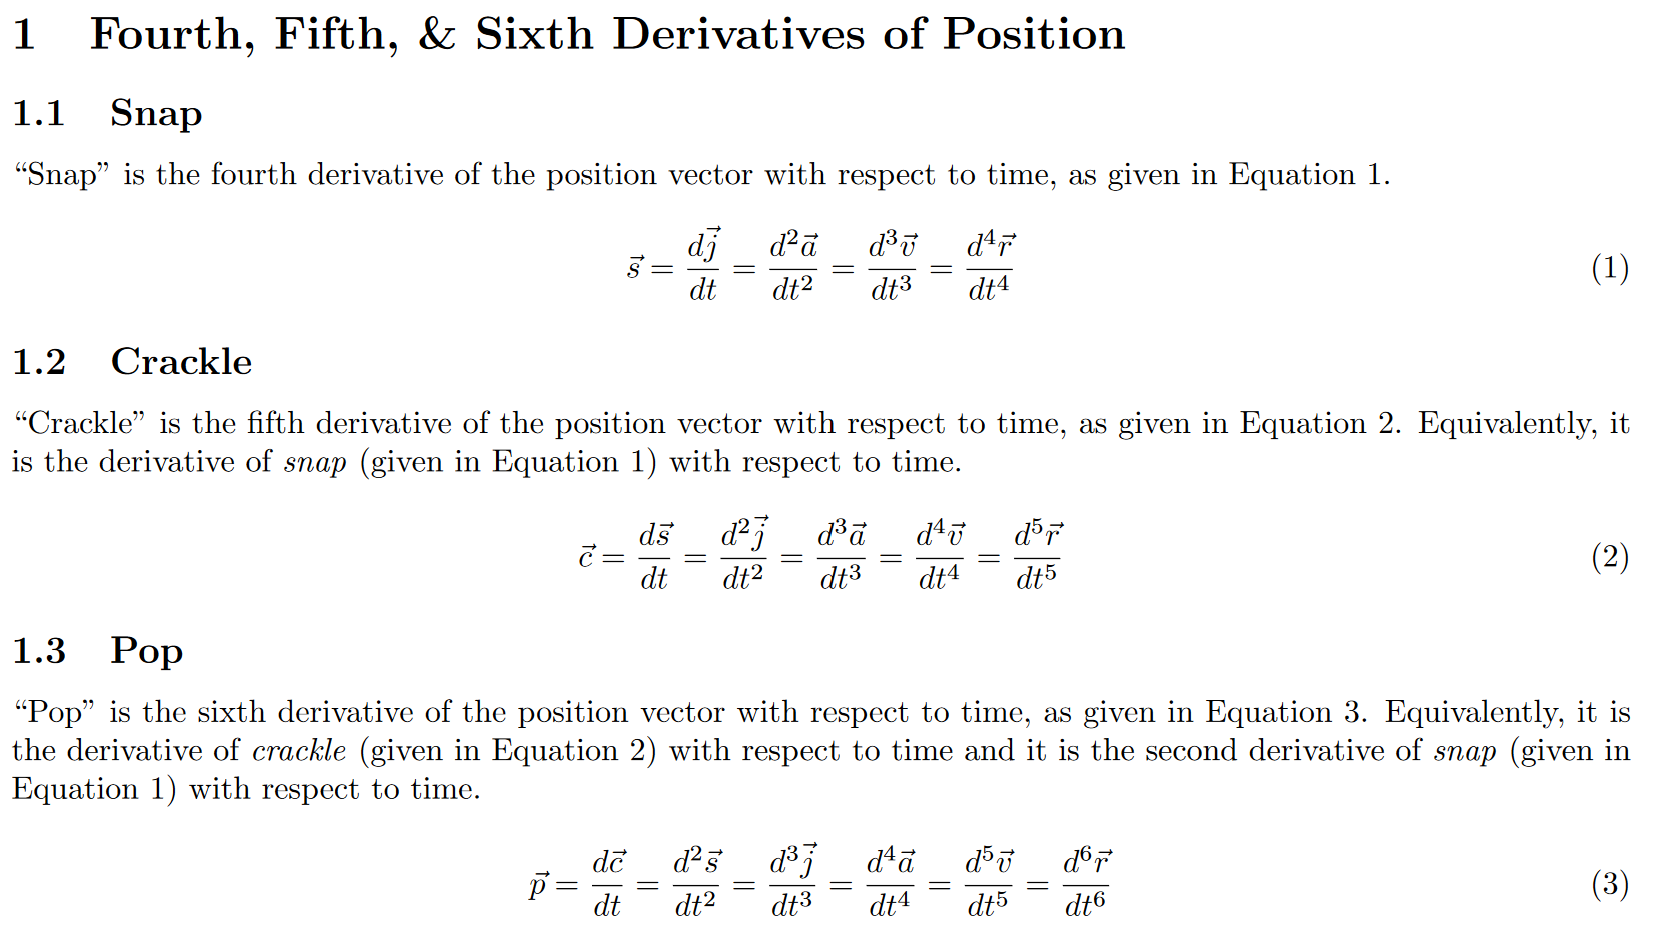
\includegraphics[width=\linewidth]{img/cereal.png}
\end{frame}


\begin{frame}[fragile]
\frametitle{Challenge: Cross-References}
\begin{alertblock}{Cross-References Source Code (1/3)}
\small
\begin{minted}{latex}
\section{Fourth, Fifth, \& Sixth Derivatives of Position}

\subsection{Snap} \label{sec:snap}

``Snap" is the fourth derivative of the position vector 
with respect to time, as given in Equation~\ref{eq:snap}.

\begin{equation} \label{eq:snap}
    \Vec{s} 
    = \frac{d\Vec{j}}{dt} = \frac{d^2 \Vec{a}}{dt^2} 
    = \frac{d^3 \Vec{v}}{dt^3} = \frac{d^4 \Vec{r}}{dt^4}
\end{equation}
\end{minted}
\end{alertblock} 
\end{frame}


\begin{frame}[fragile]
\frametitle{Challenge: Cross-References}
\begin{alertblock}{Cross-References Source Code (2/3)}
\small
\begin{minted}{latex}
\subsection{Crackle} \label{sec:crackle}

``Crackle" is the fifth derivative of the position vector 
with respect to time, as given in 
Equation~\ref{eq:crackle}. Equivalently, it is the 
derivative of \emph{snap} (given in Equation~\ref{eq:snap}) 
with respect to time.

\begin{equation} \label{eq:crackle}
    \Vec{c} 
    = \frac{d\Vec{s}}{dt} = \frac{d^2 \Vec{j}}{dt^2} 
    = \frac{d^3 \Vec{a}}{dt^3} = \frac{d^4 \Vec{v}}{dt^4} 
    = \frac{d^5 \Vec{r}}{dt^5}
\end{equation}
\end{minted}
\end{alertblock} 
\end{frame}


\begin{frame}[fragile]
\frametitle{Challenge: Cross-References}
\begin{alertblock}{Cross-References Source Code (3/3)}
\small
\begin{minted}{latex}
\subsection{Pop} \label{sec:pop}

``Pop" is the sixth derivative of the position vector with
respect to time, as given in Equation~\ref{eq:pop}. 
Equivalently, it is the derivative of \emph{crackle} 
(given in Equation~\ref{eq:crackle}) with respect to time 
and it is the second derivative of \emph{snap} (given in 
Equation~\ref{eq:snap}) with respect to time. 

\begin{equation} \label{eq:pop}
    \Vec{p} 
    = \frac{d\Vec{c}}{dt} = \frac{d^2 \Vec{s}}{dt^2} 
    = \frac{d^3 \Vec{j}}{dt^3} = \frac{d^4 \Vec{a}}{dt^4} 
    = \frac{d^5 \Vec{v}}{dt^5} = \frac{d^6 \Vec{r}}{dt^6}
\end{equation}
\end{minted}
\end{alertblock} 
\end{frame}

\section{Floats: Figures and Tables}
\begin{frame}[fragile]
\frametitle{Floats}
Tables and figures in \LaTeX{} are generally enclosed in environments called \keyw{floats}. \\[\baselineskip] \pause
\LaTeX{} automatically recognizes tables and figures, but it is also possible to define other floats. \\ \pause
\begin{block}{Definition: Floats}
    \emph{Floats} are blocks of content that ``float" around the page. They act as containers for objects in a document that should not be split up or broken over a page.
\end{block} 
\end{frame}


\begin{frame}[fragile]
\frametitle{Floats}
Floats are not part of the normal stream of text --- \LaTeX{} decides where to place them automatically using internal algorithms. \\[\baselineskip] \pause
They can be moved around by changing where they are defined in the source code or by adjusting parameters that control automatic floating. \\[\baselineskip] \pause
It is considered good practice not to change float positioning during drafting --- let \LaTeX{} position the floats first and make manual adjustments at the end of the drafting process. 
\end{frame}



\begin{frame}[fragile]
\frametitle{Figures}
    \begin{wrapfigure}{r}{0.4\textwidth}
        \centering
        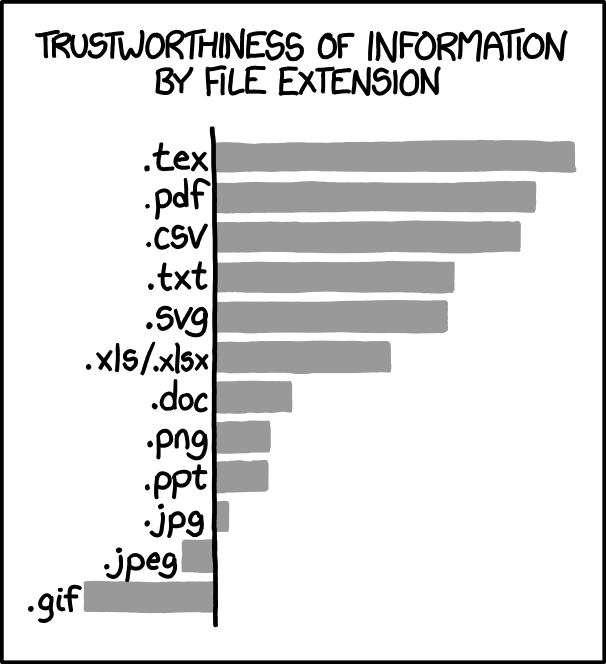
\includegraphics[width=0.35\textwidth]{img/xkcd1301_file_extensions.png}
        \caption{File Extensions}
        \label{fig:xkcd1301}
    \end{wrapfigure}
    Images are essential elements of scientific documents. \\
    Thankfully, \LaTeX{} makes them easy to manipulate with tools like... \pause
    \begin{itemize}[$\bullet$]
        \item Figures and subfigures \pause
        \item Sizing and rotating \pause
        \item Positioning (absolute or relative) \pause
        \item Captioning, labelling, and cross-referencing \pause
        \item  List of Figures
    \end{itemize}
\end{frame}
%%% wrapfigure: this command accepts two mandatory arguments: the first one is to select where we want the image, it can be r or l, that is, right or left; the second one is the width to be reserved for the image


\begin{frame}[fragile]
\frametitle{Figures: The Graphicx Package}
\LaTeX{} does not manage images by itself, so we include the \keytt{graphicx} package. \\ \pause
The \keytt{graphicx} package provides the ability to reference files from filepaths within a project. \\[\baselineskip] \pause
To load the package (in the preamble):
\begin{exampleblock}{}
    \begin{minted}{latex}
    \usepackage{graphicx}
    \end{minted}
\end{exampleblock} \pause
\vspace{0.2cm}
The most useful commands in this package are the \texttt{includegraphics} command and the \texttt{graphicspath} command:
\begin{exampleblock}{}
    \begin{minted}{latex}
    \includegraphics[keys]{filename}
    \graphicspath{ {path} }
    \end{minted}
\end{exampleblock}
\end{frame}


\begin{frame}[fragile]
\frametitle{Figures: Folders and Paths}
It is good practice to keep images in one or more separated folders so your project is organized.\\ \pause
You can tell \LaTeX{} where to look for images... \pause
\begin{block}{\small Path relative to current working directory}
\small \mintinline{latex}{ \graphicspath{ {img/} }} tells \LaTeX{} to look for images in the \texttt{img} folder relative to the current working directory.
\end{block} \pause
\begin{block}{\small Path relative to \texttt{main} file}
\small \mintinline{latex}{\graphicspath{ {./img/} }} tells \LaTeX{} to look for images in the \texttt{img} folder relative to the \texttt{main} file (denoted as \texttt{./} ).
\end{block} \pause
\small \textit{The path can also be \emph{absolute} if the exact location on your file system is specified.} \\ \pause
\textit{Or you can skip the declaration and reference the filepath directly every time instead.}
\end{frame}


\begin{frame}[fragile]
\frametitle{Figures: Positioning}

\end{frame}


\begin{frame}[fragile]
\frametitle{Figures: Positioning}
\begin{columns}
    \column{0.6\linewidth}
    The \keytt{figure} environment provides automatic positioning. 
    It uses a positioning parameter passed inside brackets. \\%\\[\baselineskip]
    \small \textit{Think of the positioning parameter as adjusting the ``settings'' on \LaTeX{}'s internal  algorithms.} \\[\baselineskip]
    \column{0.4\linewidth}
    
\includegraphics[width=\textwidth]{img/memes/hFloatFreeRealEstate.jpg}
\end{columns}
\begin{exampleblock}{}%{\small Figure Positioning Parameters}
\begin{table}[]
    \centering
    \small
    \def\arraystretch{1.25}
    \begin{tabular}{c l}
        h & ~~Place the float approximately \keyw{here}. \\
        \hline
        t & ~~Position at the \keyw{top} of the page. \\
        \hline
        b & ~~Position at the \keyw{bottom} of the page. \\
        \hline
        p & ~~Put on a special \keyw{page} for floats only.  \\
        \hline
        ! & ~~Override internal \LaTeX{} parameters. \\
        \hline
        H & ~~Place the float exactly \keyw{here}. (Similar to ``h!'')
    \end{tabular}
    % \caption{Figure Positioning Parameters}
\end{table}
\end{exampleblock}
\end{frame}





\begin{frame}[fragile]
\frametitle{Figures: Captioning, Labeling, and Cross-Referencing}
\end{frame}


\begin{frame}[fragile]
\frametitle{Figures: List of Figures}
\end{frame}


\begin{frame}[fragile]
\frametitle{Figures: Subfigures}
\end{frame}
% \begin{frame}[fragile]
\frametitle{Tables}

\end{frame}


\begin{frame}[fragile]
\frametitle{Tables: List of Tables}
    
\end{frame}


% \section{Bibliography Management}
% \input{Source-Slides/BmrSections/Bibliography.tex}


% \section{Advanced Packages (that you should know!)}
% \begin{frame}[fragile]
\frametitle{The Tikz Package}
    
\end{frame}
% \begin{frame}[fragile]
\frametitle{Beamer}

\end{frame}


\begin{frame}[fragile]
\frametitle{Beamer: }
    
\end{frame}


% \section{Field-Specific Tools}
% \begin{frame}
\frametitle{Mathematics}
    
\end{frame}


\begin{frame}
\frametitle{Theorems and Proofs}
    
\end{frame}
% \begin{frame}
\frametitle{Physics}
    
\end{frame}


\begin{frame}
\frametitle{Physics: Feynman Diagrams}
    
\end{frame}
% \begin{frame}
\frametitle{Chemistry}
    
\end{frame}


\begin{frame}
\frametitle{Chemistry Formulae}
    
\end{frame}
% \begin{frame}
\frametitle{Computer Science}
    
\end{frame}


\begin{frame}
\frametitle{Computer Science: \texttt{minted} Package}
    
\end{frame}
% \begin{frame}
\frametitle{Engineering}
    
\end{frame}
% \begin{frame}
\frametitle{Typesetting Exams}
    
\end{frame}
% \begin{frame}
\frametitle{Chess Notation}
    
\end{frame}

% \section{Resources}
% \frame{
\frametitle{Resources}
    \begin{itemize}
        \item \textbf{Overleaf} (for cloud-based editing)
        \begin{itemize}
            \item \url{https://www.overleaf.com}
        \end{itemize}
        \item \textbf{TEX Stack Exchange Forum}
        \begin{itemize}
            \item \url{https://tex.stackexchange.com/}
        \end{itemize}
        \item \textbf{Comprehensive TEX Archive Network (CTAN)}
        \begin{itemize}
            \item \url{https://ctan.org/}
        \end{itemize}
    \end{itemize}
    
    
    

}


% \input{Samples.tex}

\end{document}